% ============================================================================
% MASTER THESIS DOCUMENT
% Title: Image Encryption using Exponential Chaotic Systems
% Language: Persian (RTL)
% ============================================================================

\documentclass[a4paper,12pt]{report}
\usepackage[numbers,square]{natbib}
\usepackage{amsmath, amssymb, amsthm}

% ============================================================================
% BIDI & XEPERSUAN COMPATIBILITY FIXES (For 2024/2025 LaTeX Kernel)
% ============================================================================
\makeatletter
\providecommand{\IfFileLoadedTF}[3]{\@ifundefined{ver@#1}{#3}{#2}}
\providecommand{\IfFileLoadedF}[2]{\@ifundefined{ver@#1}{#2}{}}
\providecommand{\IfFileLoadedT}[2]{\@ifundefined{ver@#1}{}{#2}}
\providecommand{\IfPackageLoadedTF}[3]{\@ifpackageloaded{#1}{#2}{#3}}
\providecommand{\IfPackageLoadedF}[2]{\@ifpackageloaded{#1}{}{#2}}
\providecommand{\IfPackageLoadedT}[2]{\@ifpackageloaded{#1}{#2}{}}
\providecommand{\IfClassLoadedTF}[3]{\@ifclassloaded{#1}{#2}{#3}}
\providecommand{\IfClassLoadedF}[2]{\@ifclassloaded{#1}{}{#2}}
\providecommand{\IfClassLoadedT}[2]{\@ifclassloaded{#1}{#2}{}}
\makeatother

\usepackage{expl3}
\ExplSyntaxOn
% Force-define hyperref variables that are being lost/corrupted in 2024 kernel + xepersian
\int_if_exist:NF \g__hyp_link_int { \int_new:N \g__hyp_link_int }
\int_if_exist:NF \g__hyp_linknestlevel_int { \int_new:N \g__hyp_linknestlevel_int }
\bool_if_exist:NF \l__hyp_annot_GoTo_bool { \bool_new:N \l__hyp_annot_GoTo_bool }
\ExplSyntaxOff
% ============================================================================

\usepackage{graphicx}
\usepackage{subcaption}
\usepackage{xcolor}
\usepackage{tikz}
\usepackage{listings}

% listings configuration for Python
\lstset{
  language=Python,
  basicstyle=\ttfamily\small,
  keywordstyle=\color{blue},
  stringstyle=\color{red},
  commentstyle=\color{green!60!black},
  numbers=left,
  numberstyle=\tiny\color{gray},
  stepnumber=1,
  numbersep=10pt,
  backgroundcolor=\color{white},
  showspaces=false,
  showstringspaces=false,
  showtabs=false,
  frame=single,
  rulecolor=\color{black},
  tabsize=4,
  captionpos=b,
  breaklines=true,
  breakatwhitespace=false
}

\usepackage[unicode=true,hidelinks]{hyperref}
\usepackage{iftex}

\ifXeTeX
  \usepackage{fontspec}
  \usepackage[mathdigits=default]{xepersian}
  \setlatintextfont[Scale=1.0]{Times New Roman} % 12pt (matches 12pt document base)
  % Body: B Lotus (Nazok) 14pt -> Scale 1.166
  \settextfont[Scale=1.166,BoldFont={BLotusBd.ttf},ItalicFont={BLotus.ttf}]{BLotus.ttf}
  \settextdigitfont[Scale=1.166,Mapping=persian-digits]{BLotus.ttf}
  
  % Fix for B Lotus missing Persian math symbols (U+066A, U+066B)
  \makeatletter
  % Handle math mode percent
  \@ifundefined{thePersianMathPercentSymbol}{}{
    \renewcommand{\thePersianMathPercentSymbol}{\text{\lr{\%}}}
  }
  % Handle text mode percent (redefine \% to always use Latin font for the glyph)
  \let\oldpercent\%
  \renewcommand{\%}{\lr{\oldpercent}}
  % Redefine math decimal separator to standard slash (/) since B Lotus lacks U+066B (٫)
  \def\decimalseparator{/}
  \makeatother

  % Custom font sizes for headers and captions
  \usepackage{caption}
  % Captions: B Lotus Light 11pt -> Scale 11/12 = 0.916
  \DeclareCaptionFont{persianfont}{\settextfont[Scale=0.916]{BLotus.ttf}} 
  \captionsetup{font={small,persianfont}, labelfont={bf,persianfont}}
  \captionsetup[figure]{position=bottom}
  \captionsetup[table]{position=top}
  
  \SepMark{-}
  \renewcommand{\labelitemi}{$\bullet$}
\else
  \usepackage[T1]{fontenc}
  \usepackage[utf8]{inputenc}
  % Compatibility macros for xepersian commands when compiled with standard LaTeX engines
  \providecommand{\lr}[1]{#1}
  \providecommand{\LTRfootnote}[1]{\footnote{#1}}
\fi

\usepackage[top=3cm,bottom=3cm,left=2cm,right=3cm,footskip=1.5cm]{geometry}
\linespread{1.0}

% Heading styles (Bold 14pt)
\usepackage{titlesec}
\titleformat{\chapter}[display]
  {\normalfont\bfseries\huge\centering}{\chaptername\ \thechapter}{20pt}{\Huge}
\titleformat{\section}
  {\normalfont\bfseries\large}{\thesection}{1em}{}
\titleformat{\subsection}
  {\normalfont\bfseries\normalsize}{\thesubsection}{1em}{}

\usepackage{chngcntr}
\counterwithin{equation}{chapter}
\counterwithin{figure}{chapter}
\counterwithin{table}{chapter}

\author{}
\date{}


\begin{document}

% ============================================================================
% SECTION 1: TITLE PAGE & PRELIMINARY (Abjad numbering)
% ============================================================================
\pagenumbering{abjad}
% ============================================================================
% TITLE PAGE
% ============================================================================

\begin{titlepage}
\begin{center}
    
\includegraphics[width=3cm]{iau_logo} \\
    \vspace{0.5cm}
    \textbf{\Large دانشگاه آزاد اسلامی واحد بندرعباس} \\
    \textbf{\large دانشکده مهندسی کامپیوتر و فناوری اطلاعات} \\
    \vspace{1.5cm}
    \textbf{\huge پایان‌نامه برای دریافت درجه کارشناسی ارشد در رشته مهندسی کامپیوتر} \\
    \vspace{0.5cm}
    \textbf{\Large گرایش نرم‌افزار} \\
    \vspace{1.5cm}
    \textbf{\huge رمزنگاری تصاویر رنگی با استفاده از ترکیب سیستم‌های آشوبناک مبتنی بر سیستم آشوب نمایی} \\
    \vspace{2cm}
    \textbf{\Large نگارش:} \\
    \textbf{\Large منصور زاهدی} \\
    \vspace{1cm}
    \textbf{\Large استاد راهنما:} \\
    \textbf{\Large دکتر حبیب خدادادی} \\
    \vfill
    \textbf{\Large ۱۴۰۵ (تابستان)}
\end{center}
\end{titlepage}

\newpage
\setcounter{page}{2}

% ============================================================================
% BISMILLAH PAGE
% ============================================================================
\thispagestyle{empty}
\begin{center}
    \vspace*{\fill}
    {\huge بسم الله الرحمن الرحیم}
    \vspace*{\fill}
\end{center}
\newpage
      % ا (الف)
\chapter*{صورت‌جلسه دفاع از پایان‌نامه}

بدین‌وسیله گواهی می‌شود که پایان‌نامه کارشناسی‌ارشد آقای \textbf{منصور زاهدی} با عنوان:
\begin{center}
\textbf{«رمزنگاری تصاویر رنگی با استفاده از ترکیب سیستم‌های آشوبناک مبتنی بر سیستم آشوب نمایی»}
\end{center}
در تاریخ ......................... توسط هیئت داوران مورد بررسی و ارزیابی قرار گرفت و با درجه ......................... و نمره ......................... مورد تصویب نهایی قرار گرفت.

\vspace{2cm}

\begin{center}
\begin{tabular}{ccc}
\textbf{نام و نام خانوادگی} & \textbf{سمت} & \textbf{امضا} \\ \hline
......................... & استاد راهنما & ......................... \\
......................... & استاد داور داخلی & ......................... \\
......................... & استاد داور خارجی & ......................... \\
......................... & مدیر گروه & ......................... \\
\end{tabular}
\end{center}

\newpage
          % ب (Jury approval)
\chapter*{تعهدنامه اصالت رساله یا پایان‌نامه تحصیلی}

اینجانب \textbf{منصور زاهدی} دانش‌آموخته مقطع کارشناسی‌ارشد در رشته \textbf{مهندسی کامپیوتر - نرم‌افزار} که در تاریخ ......................... از پایان‌نامه خود تحت عنوان:
\begin{center}
\textbf{«رمزنگاری تصاویر رنگی با استفاده از ترکیب سیستم‌های آشوبناک مبتنی بر سیستم آشوب نمایی»}
\end{center}
با کسب نمره ............. و درجه ............................. دفاع نموده‌ام، بدین‌وسیله متعهد می‌شوم:

\begin{enumerate}
    \item این پایان‌نامه حاصل تحقیق و پژوهش انجام‌شده توسط اینجانب بوده و در مواردی که از دستاوردهای علمی و پژوهشی دیگران (اعم از پایان‌نامه، کتاب، مقاله و ...) استفاده نموده‌ام، مطابق ضوابط و رویه موجود، نام منبع مورد استفاده و سایر مشخصات آن را در فهرست مربوطه ذکر و درج کرده‌ام.
    \item این پایان‌نامه قبلاً برای دریافت هیچ مدرک تحصیلی (هم‌سطح، پایین‌تر یا بالاتر) در سایر دانشگاه‌ها و مؤسسات آموزش عالی ارائه نشده است.
    \item چنانچه بعد از فراغت از تحصیل، قصد استفاده و هرگونه بهره‌برداری اعم از چاپ کتاب، ثبت اختراع و ... از این پایان‌نامه داشته باشم، از حوزه معاونت پژوهشی واحد مجوزهای مربوطه را اخذ نمایم.
    \item چنانچه در هر مقطع زمانی خلاف موارد فوق ثابت شود، عواقب ناشی از آن را می‌پذیرم و دانشگاه آزاد اسلامی واحد بندرعباس مجاز است با اینجانب مطابق ضوابط و مقررات رفتار نموده و در صورت ابطال مدرک تحصیلی‌ام، هیچ‌گونه ادعایی نخواهم داشت.
\end{enumerate}

\vspace{1cm}

\begin{flushleft}
\begin{tabular}{l}
\textbf{نام و نام خانوادگی دانشجو:} منصور زاهدی \\
\textbf{تاریخ:} ......................... \\
\textbf{امضا:} ......................... \\
\end{tabular}
\end{flushleft}

\newpage
   % ج (Authenticity undertaking)
\chapter*{منشور اخلاق پژوهش}

با یاری از خداوند سبحان و اعتقاد به اینکه عالم محضر خداست و همواره ناظر بر اعمال انسان و به منظور پاس‌داشت مقام بلند دانش و پژوهش و نظر به اهمیت جایگاه دانشگاه در اعتلای فرهنگ و تمدن بشری، ما دانشجویان و اعضای هیئت علمی واحدهای دانشگاه آزاد اسلامی متعهد می‌گردیم اصول زیر را در انجام فعالیت‌های پژوهشی مدنظر قرار داده و از آن تخطی نکنیم:

\begin{enumerate}
    \item \textbf{اصل حقیقت‌جویی:} تلاش در راستای پی‌جویی حقیقت و وفاداری به آن و دوری از هرگونه پنهان‌سازی حقیقت.
    \item \textbf{اصل رعایت حقوق:} التزام به رعایت کامل حقوق پژوهشگران و پژوهیدگان (انسان، حیوان و نبات) و سایر صاحبان حق.
    \item \textbf{اصل مالکیت مادی و معنوی:} تعهد به رعایت کامل حقوق مادی و معنوی دانشگاه و کلیه همکاران پژوهش.
    \item \textbf{اصل منافع ملی:} تعهد به رعایت مصالح ملی و در نظر داشتن پیشبرد و توسعه کشور در کلیه مراحل پژوهش.
    \item \textbf{اصل رعایت انصاف و امانت:} تعهد به اجتناب از هرگونه جانبداری غیرعلمی و حفاظت از اموال، تجهیزات و منابع در اختیار.
    \item \textbf{اصل رازداری:} تعهد به صیانت از اسرار و اطلاعات محرمانه افراد، سازمان‌ها، کشور و کلیه افراد و نهادهای مرتبط با تحقیق.
    \item \textbf{اصل احترام:} تعهد به رعایت حریم‌ها و حرمت‌ها در انجام تحقیقات و رعایت جانب نقد و خودداری از هرگونه حرمت‌شکنی.
    \item \textbf{اصل ترویج:} تعهد به رواج دانش و اشاعه نتایج تحقیقات و انتقال آن به همکاران علمی و دانشجویان، به غیر از مواردی که منع قانونی دارد.
    \item \textbf{اصل برائت:} التزام به برائت‌جویی از هرگونه رفتار غیرحرفه‌ای و اعلام موضع نسبت به کسانی که حوزه علم و پژوهش را به شائبه‌های غیرعلمی می‌آلایند.
\end{enumerate}

\vspace{1cm}

\begin{flushleft}
\begin{tabular}{l}
\textbf{نام و نام خانوادگی دانشجو:} منصور زاهدی \\
\textbf{تاریخ:} ......................... \\
\textbf{امضا:} ......................... \\
\end{tabular}
\end{flushleft}

\newpage
        % د (Research ethics)
\chapter*{تقدیم}
این اثر به خانواده عزیزم تقدیم می‌شود.
\newpage
    % هـ (Dedication)
\chapter*{سپاسگزاری}
از اساتید راهنما و تمامی کسانی که مرا در این راه یاری کردند سپاسگزاری می‌کنم.
\newpage
 % و (Acknowledgments)
% ============================================================================
% TABLE OF CONTENTS, TABLES, AND FIGURES
% ============================================================================
\begin{NoHyper}
\tableofcontents
\clearpage
\addcontentsline{toc}{chapter}{\listtablename}
\listoftables
\clearpage
\addcontentsline{toc}{chapter}{\listfigurename}
\listoffigures
\end{NoHyper}
\clearpage
   % ز، ح، ط (TOC, LOT, LOF)
\chapter*{فهرست اختصارات و علائم}
\addcontentsline{toc}{chapter}{فهرست اختصارات و علائم}
\begin{latin}
\begin{itemize}
    \item[DNA] Deoxyribonucleic Acid
    \item[MD5] Message Digest 5
    \item[NPCR] Number of Pixel Change Rate
    \item[UACI] Unified Average Changing Intensity
    \item[RGB] Red, Green, Blue
    \item[MSE] Mean Squared Error
    \item[PSNR] Peak Signal-to-Noise Ratio
    \item[PRNG] Pseudo-Random Number Generator
    \item[NIST] National Institute of Standards and Technology
    \item[SSIM] Structural Similarity Index Measure
\end{itemize}
\end{latin}
\newpage
 % ي (Abbreviations)
\clearpage

% ============================================================================
% SECTION 2: ABSTRACT & CHAPTERS
% ============================================================================
\pagenumbering{arabic}
\setcounter{page}{1}
% ============================================================================
% PERSIAN ABSTRACT
% ============================================================================

\chapter*{چکیده}

\textbf{هدف:} هدف اصلی این پژوهش، افزایش امنیت و کارایی رمزنگاری تصاویر با ایجاد پیچیدگی بیشتر و کاهش همبستگی پیکسل‌ها از طریق ترکیب سیستم‌های آشوبی نمایی (\lr{ECM}) و سیستم آشوبی سه‌بعدی \lr{Chen} است. 
\textbf{روش:} الگوریتم پیشنهادی شامل دو مرحله اصلی جایگشت (با استفاده از سیستم \lr{Chen}) و انتشار (با انتخاب تصادفی یکی از 9 سیستم نمایی برای هر پیکسل) می‌باشد. پیاده‌سازی در محیط \lr{Python} و ارزیابی بر روی تصاویر استاندارد \lr{USC-SIPI} انجام شده است. 
\textbf{نتایج:} نتایج تحلیل‌های امنیتی نشان می‌دهد که آنتروپی تصاویر رمز شده به‌طور میانگین به 7.9993 بیت رسیده و همبستگی پیکسل‌های مجاور از میانگین 0.9989 در تصاویر اصلی به 0.0126 در تصاویر رمزنگاری‌شده کاهش یافته است که معادل کاهش \lr{98.7\%} است. همچنین مقادیر \lr{NPCR} و \lr{UACI} به ترتیب \lr{94.91\%} و \lr{30.19\%} محاسبه شده که نشان‌دهنده مقاومت بالا در برابر حملات است. زمان اجرای الگوریتم برای تصاویر 512 × 512 حدود 26.22 ثانیه است. 
\textbf{نتیجه‌گیری:} نوآوری در انتخاب دینامیک سیستم نمایی برای هر پیکسل و استفاده ترکیبی از سیستم \lr{Chen}، توازن مناسبی بین امنیت و سرعت ایجاد کرده و این روش را برای کاربردهای بلادرنگ مناسب می‌سازد.
    
    \vspace{1cm}
    \textbf{کلیدواژه‌ها:} رمزنگاری تصویر، سیستم‌های آشوبی نمایی، سیستم چن، آنتروپی شانون، جایگشت و انتشار.
    \newpage


% ============================================================================
% CHAPTER 1: INTRODUCTION AND RESEARCH SPECIFICATIONS
% ============================================================================

\chapter{کلیات تحقیق}

\section{بیان مسئله}
در عصر دیجیتال، تبادل اطلاعات به‌ویژه در قالب تصاویر، به بخشی جدایی‌ناپذیر از ارتباطات، تجارت، سیستم‌های نظارتی و رسانه‌های اجتماعی تبدیل شده است. در این میان، تصاویر دیجیتال به دلیل نقش کلیدی در انتقال داده‌های بصری، به یکی از مهم‌ترین انواع اطلاعات چندرسانه‌ای بدل شده‌اند که حجم بالایی از داده را در خود جای می‌دهند و کاربرد گسترده‌ای در شبکه‌های ارتباطی، سامانه‌های ذخیره‌سازی و تحلیل داده دارند \cite{ref1}.

با گسترش دسترسی به فضای مجازی و تهدیدهای فزاینده در حوزه امنیت سایبری، حفاظت از حریم خصوصی اطلاعات تصویری به یکی از دغدغه‌های اصلی پژوهشگران و توسعه‌دهندگان امنیت اطلاعات تبدیل شده است. برخلاف داده‌های متنی که رمزنگاری آن‌ها با الگوریتم‌های استانداردی نظیر \lr{AES} و \lr{RSA} به‌خوبی قابل انجام است، تصاویر دیجیتال به دلیل ویژگی‌هایی همچون حجم زیاد، ساختار دوبعدی، همبستگی آماری بالا میان پیکسل‌های مجاور و حساسیت بالا به تغییرات، به الگوریتم‌های رمزنگاری تخصصی‌تر و پیچیده‌تری نیاز دارند \cite{ref2, ref3}.

مهم‌ترین چالش‌ها در رمزنگاری تصاویر دیجیتال را می‌توان به شرح زیر برشمرد:
\begin{itemize}
    \item حفظ ویژگی‌های آماری تصویر پس از رمزنگاری؛
    \item ایجاد مقاومت در برابر انواع حملات نظیر تحلیل آماری، حملات تمایزی و جستجوی فراگیر\LTRfootnote{Brute Force}؛
    \item کاهش بار محاسباتی جهت کاربرد در سامانه‌های بلادرنگ؛
    \item پیشگیری از تخریب داده‌های تصویری طی فرآیند رمزنگاری و رمزگشایی.
\end{itemize}

در پاسخ به این چالش‌ها، بهره‌گیری از سیستم‌های آشوبی\LTRfootnote{Chaotic Systems} به‌عنوان راهکاری مؤثر مورد توجه قرار گرفته است. سیستم‌های آشوبی با رفتار غیرخطی، حساسیت شدید به شرایط اولیه و توانایی تولید دنباله‌های شبه‌تصادفی، امکان طراحی الگوریتم‌هایی با امنیت بالا و کلیدهای غیرقابل پیش‌بینی را فراهم می‌آورند \cite{ref4}. فرآیندهای جایگشت\LTRfootnote{Permutation} و پراکندگی پیکسل‌ها با کمک این سیستم‌ها، ساختار آماری تصویر را به‌شدت تغییر داده و مانع بازیابی تصویر اصلی بدون کلید می‌شوند.

با این حال، یکی از نقاط ضعف رایج در الگوریتم‌های مبتنی بر سیستم‌های آشوبی کلاسیک، بروز پدیده‌ای به‌نام «تخریب آشوب»\LTRfootnote{Chaotic Degradation} است. این پدیده در شرایط خاص یا در اثر خطای عددی می‌تواند باعث از دست رفتن ویژگی‌های آشوبی شود و در نهایت، امنیت سیستم را کاهش دهد. این اشکال به‌ویژه در سیستم‌هایی نظیر سیستم لجستیک\LTRfootnote{Logistic} و تنت\LTRfootnote{Tent} به‌صورت برجسته‌تری مشاهده شده است \cite{ref5}.

سیستم آشوبی به‌طور کلی، نوعی سیستم دینامیکی غیرخطی است که رفتار آن در طول زمان به شدت به شرایط اولیه وابسته است و این وابستگی منجر به تولید پاسخ‌هایی کاملاً متفاوت در صورت تغییرات بسیار جزئی در مقدارهای ورودی می‌شود. به بیان ساده‌تر، سیستم آشوبی با وجود پیروی از معادلات مشخص، خروجی‌ای شبه‌تصادفی و غیرقابل پیش‌بینی تولید می‌کند، به‌گونه‌ای که برای ناظر بیرونی همانند نویز یا تصادف به نظر می‌رسد، اما در واقع دارای نظم در بی‌نظمی‌است.

ویژگی‌های اصلی سیستم‌های آشوبی شامل:
\begin{itemize}
    \item حساسیت شدید به شرایط اولیه \LTRfootnote{Sensitive Dependence on Initial Conditions}
    \item غیرخطی بودن روابط سیستم \LTRfootnote{Nonlinearity}
    \item رفتار شبه‌تصادفی \LTRfootnote{Pseudo-randomness}
    \item وابستگی به پارامترهای سیستمی
\end{itemize}

این ویژگی‌ها باعث می‌شوند که سیستم‌های آشوبی گزینه‌ای بسیار مناسب برای تولید کلیدهای رمزنگاری، الگوریتم‌های پراکندگی و اختفاء داده‌ها باشند. به‌عنوان مثال، سیستم‌های ساده‌ای مانند لجستیک، تنت، هنون\LTRfootnote{Henon}، چن\LTRfootnote{Chen} و لورنز\LTRfootnote{Lorenz} به‌طور گسترده در رمزنگاری تصویر به‌کار رفته‌اند. سیستم لورنز (\lr{Lorenz system}) یکی از مشهورترین مدل‌های آشوبی سه‌بعدی است که از معادلات دیفرانسیل غیرخطی تشکیل شده و در ابتدا برای مدل‌سازی حرکت سیالات جوی طراحی شد، اما به‌دلیل توانایی بالا در تولید مسیرهای آشوبی، امروزه در حوزه رمزنگاری و ارتباطات امن نیز مورد استفاده قرار گرفته است \cite{ref6}.

در پژوهش حاضر، با هدف ارتقاء سطح امنیت و کارایی الگوریتم‌های رمزنگاری تصویر، روشی جدید معرفی می‌شود که از ترکیب 9 سیستم آشوبی نمایی به‌همراه الگوریتم جایگشت \lr{Chen} بهره می‌برد. سیستم‌های نمایی، مانند \lr{LEL}، \lr{SEL} و سایر سیستم‌های آشوبی نمائی، به‌عنوان نسل جدید سیستم‌های آشوبی، قادرند رفتارهای پیچیده‌تر و توزیع آماری یکنواخت‌تری نسبت به مدل‌های کلاسیک ایجاد کنند \cite{ref4}.

در این الگوریتم، ابتدا پیکسل‌های تصویر با استفاده از دنباله‌های تولیدشده توسط سیستم \lr{Chen} به‌صورت تصادفی جابه‌جا می‌شوند. سپس، رمزنگاری هر پیکسل با انتخاب تصادفی یکی از 9 سیستم نمایی صورت می‌گیرد. این رویکرد چندلایه، علاوه بر ارتقاء پیچیدگی، موجب افزایش آنتروپی اطلاعاتی، کاهش همبستگی پیکسل‌ها و افزایش مقاومت در برابر حملات تحلیل آماری می‌شود. از طرفی، با بهره‌گیری از توزیع‌های آماری غیرخطی‌تر و پایدارتر، احتمال تخریب ویژگی‌های آشوبی به‌طور مؤثری کاهش می‌یابد.

در نهایت، هدف از این تحقیق، توسعه یک الگوریتم رمزنگاری مقاوم و کارآمد است که با تکیه بر سیستم‌های آشوبی نوین، توازنی بهینه میان امنیت بالا و سرعت اجرای مناسب برقرار کرده و پاسخگوی نیازهای کاربردی در حوزه‌هایی همچون پزشکی، امنیت نظامی، شبکه‌های اجتماعی و ذخیره‌سازی ابری باشد.

\section{اهمیت و ضرورت تحقیق}
با گسترش فناوری‌های دیجیتال و افزایش وابستگی جوامع به سامانه‌های الکترونیکی، امنیت اطلاعات به یکی از دغدغه‌های اصلی در حوزه فناوری اطلاعات تبدیل شده است. تصاویر دیجیتال، به‌ویژه تصاویر رنگی\LTRfootnote{Color Images}، به‌دلیل حجم بالای اطلاعات و کاربرد گسترده در حوزه‌هایی مانند ارتباطات، شبکه‌های اجتماعی، نظارت تصویری، پزشکی و نظامی، بیش از گذشته در معرض تهدیدات امنیتی نظیر شنود، جعل و دستکاری قرار دارند \cite{ref10}. اهمیت حفاظت از این داده‌های بصری، ضرورت توسعه روش‌های نوین رمزنگاری را دوچندان کرده است.

یکی از چالش‌های اساسی در رمزنگاری تصاویر رنگی، ساختار پیچیده و چندبعدی آن‌هاست. تصاویر رنگی به‌صورت ترکیبی از سه کانال \lr{RGB} تعریف می‌شوند که وابستگی بین کانال‌ها، کار رمزنگاری ایمن و بهینه را دشوار می‌سازد. این وابستگی‌ها می‌توانند توسط مهاجمان برای تحلیل ساختاری تصویر مورد سوءاستفاده قرار گیرند \cite{ref3}. بنابراین، طراحی الگوریتم‌هایی که بتوانند این وابستگی‌ها را کاهش داده و توزیع داده‌ها را تصادفی‌تر سازند، امری حیاتی به نظر می‌رسد.

مطالعات متعددی در حوزه رمزنگاری آشوبی انجام شده‌اند که نشان می‌دهند سیستم‌های آشوبی به‌دلیل ویژگی‌هایی نظیر حساسیت بالا به شرایط اولیه، رفتار غیرخطی و قابلیت تولید دنباله‌های شبه‌تصادفی پیچیده، ظرفیت بالایی در تولید کلیدهای رمزنگاری غیرقابل پیش‌بینی دارند. با این حال، اغلب روش‌های موجود تنها از یک سیستم آشوبی منفرد استفاده می‌کنند که در برابر حملاتی مانند تحلیل همبستگی و جستجوی فراگیر آسیب‌پذیر هستند \cite{ref12}. به‌منظور مقابله با این آسیب‌پذیری‌ها، استفاده از ترکیب چند سیستم آشوبی نمایی به‌صورت تصادفی، می‌تواند پیچیدگی رمزنگاری را افزایش داده و مقاومت آن را در برابر انواع حملات ارتقا بخشد.

بر اساس یافته‌های اخیر، سیستم‌های آشوبی نمایی نسبت به سیستم‌های آشوبی کلاسیک مانند سیستم لجستیک و سیستم تنت، توزیع احتمال پیچیده‌تری تولید می‌کنند و پایداری بیشتری در برابر تغییرات پارامترها دارند. این ویژگی‌ها آن‌ها را به گزینه‌ای مناسب برای پیاده‌سازی رمزنگاری‌های مقاوم تبدیل کرده است \cite{ref5}. از طرف دیگر، استفاده از سیستم‌هایی نظیر سیستم آشوبی چن، با ویژگی‌هایی همچون سرعت پردازش بالا و سادگی پیاده‌سازی، می‌توانند به افزایش کارایی الگوریتم‌های رمزنگاری کمک کنند.

افزون بر این، بسیاری از کاربردهای حیاتی نظیر انتقال تصاویر پزشکی، داده‌های مالی در بانکداری، یا اطلاعات طبقه‌بندی‌شده در صنایع نظامی، نیازمند الگوریتم‌هایی هستند که هم امنیت بسیار بالایی داشته باشند و هم بتوانند در زمان محدود پردازش انجام دهند؛ این مسئله، لزوم دستیابی به توازنی منطقی میان امنیت و کارایی را پررنگ‌تر می‌کند \cite{ref5}. در همین راستا، پژوهش حاضر با ترکیب 9 سیستم آشوبی نمایی و استفاده از سیستم آشوبی چن جهت جایگشت، در پی توسعه مدلی نوین است که بتواند این توازن را به‌صورت مؤثر محقق سازد.

در نهایت، رمزنگاری آشوبی به‌عنوان یکی از حوزه‌های نوظهور در علوم رمزنگاری، همچنان نیازمند تحقیقات عمیق‌تری برای بهره‌برداری کامل از ظرفیت‌های خود است. مطالعات نظری و تجربی در این زمینه می‌توانند زمینه‌ساز توسعه مدل‌های امن‌تر و بهینه‌تری برای محافظت از داده‌های حساس در عصر دیجیتال باشند. پژوهش حاضر، با تمرکز بر طراحی و ارزیابی یک روش ترکیبی پیشرفته، می‌کوشد گامی‌مؤثر در مسیر توسعه دانش رمزنگاری آشوبی بردارد.

\section{اهداف تحقیق}
\subsection{هدف کلی}
طراحی و توسعه‌ی الگوریتمی‌برای رمزنگاری تصاویر رنگی با بهره‌گیری از ترکیب 9 سیستم آشوبی نمایی، با هدف ارتقاء امنیت اطلاعات تصویری و بهبود کارایی محاسباتی.

\subsection{اهداف جزئی}
\begin{itemize}
    \item بررسی عملکرد 9 سیستم آشوبی نمایی در تولید دنباله‌های تصادفی پیچیده و غیرقابل پیش‌بینی.
    \item بهبود مقاومت الگوریتم رمزنگاری در برابر حملات آماری و جستجوی فراگیر از طریق ترکیب چندین سیستم آشوبی.
    \item افزایش پیچیدگی فرآیند رمزنگاری با استفاده از انتخاب تصادفی سیستم آشوبی برای رمزنگاری هر پیکسل.
    \item مقایسه امنیت و کارایی الگوریتم پیشنهادی با سایر روش‌های رمزنگاری مبتنی بر آشوب و ارزیابی میزان برتری آن.
\end{itemize}

\section{فرضیات تحقیق}
در این پژوهش، فرضیات زیر مورد بررسی و ارزیابی قرار می‌گیرند:
\begin{enumerate}
    \item استفاده از ترکیب 9 سیستم آشوبی نمایی باعث افزایش حساسیت الگوریتم به تغییرات کوچک در تصویر اصلی (\lr{Avalanche effect}) و بهبود شاخص‌های \lr{NPCR} و \lr{UACI} می‌گردد.
    \item به‌کارگیری سیستم آشوبی چن در مرحله جایگشت، همبستگی آماری میان پیکسل‌های مجاور را به حداقل ممکن (نزدیک به صفر) کاهش می‌دهد.
    \item انتخاب تصادفی سیستم آشوبی برای هر پیکسل، آنتروپی اطلاعات تصویر رمزشده را به مقدار ایده‌آل (8 بیت) نزدیک می‌کند.
    \item الگوریتم پیشنهادی علی‌رغم پیچیدگی ساختاری، از کارایی محاسباتی مطلوبی برخوردار بوده و برای کاربردهای بلادرنگ مناسب است.
    \item توزیع هیستوگرام تصاویر رمزشده به‌صورت کاملاً یکنواخت بوده و الگوریتم در برابر حملات آماری و تحلیل هیستوگرام مقاوم است.
\end{enumerate}

\section{سهم علمی‌پژوهش}
در این پایان‌نامه، یک چارچوب نوین برای رمزنگاری تصاویر رنگی مبتنی بر سیستم‌های آشوبی نمایی ارائه شده است که با هدف افزایش امنیت، پیچیدگی دینامیکی و معکوس‌پذیری کامل طراحی گردیده است. مهم‌ترین سهم‌های علمی‌این پژوهش به شرح زیر می‌باشند:
\begin{enumerate}
    \item ارائه یک الگوریتم رمزنگاری تصویر مبتنی بر مدل آشوبی نمایی\LTRfootnote{Exponential Chaotic Model} که با ترکیب غیرخطی سیستم‌های پایه، دنباله‌های آشوبی با رفتار پیچیده‌تر و حساسیت بالاتر نسبت به شرایط اولیه تولید می‌کند.
    \item استفاده همزمان از چند سیستم آشوبی نمایی (9 سیستم متفاوت) و انتخاب پویای آن‌ها در سطح پیکسل که منجر به افزایش فضای کلید، کاهش الگوپذیری و ارتقای مقاومت الگوریتم در برابر حملات آماری و دیفرانسیلی می‌شود.
    \item طراحی یک سازوکار انتشار\LTRfootnote{Diffusion} اصلاح‌شده و کاملاً معکوس‌پذیر که در آن دنباله آشوبی صرفاً به کلید و اندیس پیکسل وابسته بوده و از وابستگی مستقیم به مقدار پیکسل جلوگیری شده است. این ویژگی تضمین می‌کند که تصویر رمزگشایی‌شده به‌صورت \lr{100\%} با تصویر اصلی منطبق باشد.
    \item بهره‌گیری از سیستم آشوبی پیوسته \lr{Chen} برای تولید جریان کلید که در مقایسه با سیستم‌های گسسته، کیفیت آشوب، حساسیت به شرایط اولیه و امنیت کلید را به‌طور قابل‌توجهی افزایش می‌دهد.
    \item انجام مجموعه‌ای جامع از تحلیل‌های امنیتی شامل آنتروپی شانون\LTRfootnote{Shannon Entropy}، همبستگی پیکسل‌های مجاور، \lr{NPCR}، \lr{UACI} و تحلیل هیستوگرام که نشان‌دهنده عملکرد مناسب الگوریتم پیشنهادی در مقایسه با روش‌های موجود می‌باشد.
    \item پیاده‌سازی کامل الگوریتم و ارزیابی تجربی آن بر روی تصاویر رنگی استاندارد با ابعاد مختلف که کارایی عملی و قابلیت کاربرد الگوریتم در سناریوهای واقعی را تأیید می‌کند.
\end{enumerate}

\section{ساختار پایان‌نامه}
ساختار این پایان‌نامه به‌صورت زیر سازماندهی شده است:

\textbf{فصل دوم:} مفاهیم پایه و پیش‌نیازهای نظری مرتبط با رمزنگاری تصاویر، سیستم‌های آشوبی، ویژگی‌های سیستم‌های آشوبی و معیارهای ارزیابی امنیت مرور می‌شود. همچنین برخی از مهم‌ترین پژوهش‌های انجام‌شده در این حوزه مورد بررسی قرار می‌گیرند.

\textbf{فصل سوم:} به معرفی الگوریتم پیشنهادی اختصاص دارد. در این فصل، معماری کلی روش ارائه‌شده، فرآیند تولید کلید، مرحله جایگشت و مرحله انتشار به‌طور دقیق تشریح شده و روند رمزنگاری و رمزگشایی به‌صورت گام‌به‌گام توضیح داده می‌شود.

\textbf{فصل چهارم:} پیاده‌سازی عملی الگوریتم و نتایج آزمایش‌های تجربی ارائه می‌گردد. در این فصل، عملکرد الگوریتم پیشنهادی از نظر معیارهای امنیتی و آماری تحلیل شده و نتایج به‌صورت جداول و نمودارهای تحلیلی گزارش می‌شوند.

\textbf{فصل پنجم:} نتایج به‌دست‌آمده مورد بحث و بررسی قرار گرفته و عملکرد روش پیشنهادی با برخی از روش‌های مطرح در ادبیات پژوهش مقایسه می‌شود. در پایان این فصل، جمع‌بندی نهایی پژوهش ارائه شده و پیشنهادهایی برای تحقیقات آینده مطرح می‌گردد.

\newpage
% ============================================================================
% CHAPTER 2: BASIC CONCEPTS AND LITERATURE REVIEW
% ============================================================================

\chapter{مفاهیم پایه و پیشینه پژوهش}

\section{مقدمه}
از زمان انتشار مشاهده‌های ادوارد لورنز در زمینه‌ی رفتارهای آشوبناک، مفهوم «آشوب» به یکی از موضوعات مورد توجه در جامعه‌ی علمی‌تبدیل شد. نظریه‌ی آشوب شاخه‌ای از ریاضیات است که به تحلیل سیستم‌هایی می‌پردازد که رفتار آن‌ها به تغییرات کوچک در شرایط اولیه بسیار حساس است. به بیان دیگر، در این‌گونه سامانه‌ها، تغییرات ظاهراً ناچیز می‌تواند منجر به تفاوت‌های چشمگیر در خروجی شود.

پیش از ظهور این نظریه، بسیاری از پدیده‌های تصادفی یا غیرقابل‌پیش‌بینی، فاقد توجیه علمی‌دقیق تلقی می‌شدند. اما نظریه‌ی آشوب توانست با اتکا بر اصول ریاضی، فیزیک و فلسفه، مبانی تبیینی منسجمی‌برای این پدیده‌ها فراهم آورد. قانون علت و معلول همچنان در این نظریه برقرار است، اما تعداد عوامل مؤثر بر نتایج به‌طور چشمگیری افزایش می‌یابد. در واقع، نظریه‌ی آشوب ابزاری فراهم می‌کند تا بتوان پدیده‌های پیچیده‌ی طبیعی و واقعی را بهتر درک و تحلیل کرد.

نکته‌ی مهم آن است که نظریه‌ی آشوب صرفاً به‌منزله‌ی روشی برای ساده‌سازی پدیده‌های فیزیکی در نظر گرفته نمی‌شود. مدل‌های ریاضی ناشی از آن، به‌عنوان منبعی از اطلاعات جدید و غیرخطی محسوب می‌شوند. این مدل‌ها می‌توانند نه تنها رفتار سامانه‌های واقعی را پیش‌بینی کنند، بلکه در حوزه‌های دیگر از جمله علوم مهندسی، فیزیک و رمزنگاری اطلاعات نیز به کار گرفته شوند.

در سال‌های اخیر، توجه ویژه‌ای به کاربرد نظریه‌ی آشوب در علم ارتباطات و امنیت اطلاعات شده است. ویژگی‌هایی چون حساسیت بالا به شرایط اولیه، غیرقابل‌پیش‌بینی بودن و رفتار شبه‌تصادفی، سبب شده تا سیستم‌های آشوبی به‌عنوان بستری مناسب برای طراحی الگوریتم‌های رمزنگاری مطرح شوند.

در واقع، میان ویژگی‌های ذاتی سیستم‌های آشوبی و خواص مطلوب در یک سامانه‌ی رمزنگاری امن شباهت‌های قابل‌توجهی وجود دارد. این خواص شامل پخش و درهم‌سازی قوی، وابستگی شدید به کلید و مقاومت در برابر حملات آماری است. با وجود این ارتباط نزدیک، طراحی الگوریتم‌های رمزنگاری مؤثر نیازمند دقت و دانش عمیق ریاضی است؛ چرا که هرگونه خطا در پیاده‌سازی یا انتخاب پارامترها می‌تواند امنیت سامانه را به‌شدت کاهش دهد.

\subsection{اهداف و ساختار فصل}
در این فصل به معرفی مبانی نظری مرتبط با موضوع پژوهش پرداخته می‌شود. ابتدا مفاهیم بنیادین رمزنگاری و انواع روش‌های آن مرور می‌گردد. در ادامه ویژگی‌های اصلی تصاویر دیجیتال، نظریه‌ی آشوب، انواع توابع آشوب و ارتباط میان آشوب و رمزنگاری مورد بررسی قرار می‌گیرد. در نهایت نیز به بررسی پژوهش‌های پیشین در زمینه‌ی استفاده از سیستم‌های آشوبی در رمزنگاری تصاویر رنگی پرداخته خواهد شد.


\section{رمزنگاری}
رمزنگاری یا رمزگذاری فرآیند تبدیل اطلاعات به‌کمک یک الگوریتم خاص به صورتی غیرقابل‌فهم برای افراد غیرمجاز است. هدف از این کار، ذخیره یا انتقال امن داده‌ها و جلوگیری از دسترسی یا سوء‌استفاده‌ی احتمالی است. 

در هر سیستم رمزنگاری، کلیدی وجود دارد که تنها در اختیار رمزگذار یا گیرنده‌ی مجاز قرار دارد. این کلید برای معکوس‌سازی عملیات رمزنگاری و بازگردانی داده‌ها به حالت اولیه (رمزگشایی) به‌کار می‌رود.

رمزنگاری از دیرباز در میان دولت‌ها، نیروهای نظامی‌و نهادهای امنیتی برای برقراری ارتباطات محرمانه مورد استفاده قرار می‌گرفت. با گذشت زمان و گسترش فناوری‌های دیجیتال، کاربرد آن به حوزه‌های غیرنظامی‌نیز گسترش یافته است. امروزه در بسیاری از سامانه‌های کامپیوتری و ارتباطی، به‌منظور حفظ امنیت داده‌ها، از روش‌های رمزگذاری استفاده می‌شود. این فناوری برای محافظت از داده‌های ذخیره‌شده یا در جریان انتقال از طریق شبکه‌هایی نظیر اینترنت، تلفن همراه و ارتباطات بی‌سیم به‌کار گرفته می‌شود\cite{ref14}.

از دیدگاه واژه‌شناسی، رمزنگاری به معنای پنهان‌نویسی است. در مفهوم علمی، این حوزه شامل تبدیل متن آشکار\LTRfootnote{Plain Text} به متن رمز\LTRfootnote{Cipher Text} و برعکس است. (شکل\ref{fig:visual_results} در فصل چهارم نمونه‌هایی از این تبدیل بر روی تصاویر استاندارد را نشان می‌دهد). در دوران باستان، روش‌های ابتدایی جایگزینی حروف برای رمزگذاری پیام‌ها استفاده می‌شد. در این روش هر حرف با حرف یا نمادی دیگر جایگزین می‌شد که تنها افراد خاص از معنای آن اطلاع داشتند. با وجود کاربرد ساده، این روش با چالش‌هایی مواجه بود؛ زیرا لازم بود برای هر جفت فرستنده و گیرنده، یک مجموعه کد منحصربه‌فرد تعریف شود\cite{ref15}.

به همین دلیل، مفهوم کلید در رمزنگاری مطرح شد. در این روش، تبدیل متن آشکار به متن رمز براساس پارامتری مستقل از خود متن انجام می‌گیرد. به این ترتیب، فرستنده و گیرنده تنها لازم است از الگوریتم رمزنگاری و کلید مشترک اطلاع داشته باشند. این تحول باعث شد رمزنگاری از حوزه‌ی زبان طبیعی وارد دنیای دیجیتال شود و به شاخه‌ای از ریاضیات و علوم رایانه تبدیل گردد\cite{ref16}.

به‌طور کلی، علم رمزنگاری امروزه نقش بنیادینی در امنیت ارتباطات دیجیتال، بانکداری الکترونیک، تجارت اینترنتی، شبکه‌های اجتماعی و حتی ذخیره‌سازی ابری ایفا می‌کند و پایه‌ی بسیاری از سامانه‌های امنیتی مدرن را تشکیل می‌دهد.

\subsection{تعریف رمزنگاری}
رمزنگاری فرآیندی است که طی آن اطلاعات به‌گونه‌ای دچار تغییر و بازآرایی می‌شوند که برای افراد غیرمجاز غیرقابل فهم باشد. فناوری رمزنگاری دسترسی به پیام‌ها و اطلاعات ارسالی را برای افراد غیرمجاز محدود کرده و امکان مشاهده، مطالعه و تفسیر آن‌ها را سلب می‌کند. این فناوری به‌ویژه برای حفاظت از داده‌ها در شبکه‌های عمومی‌مانند اینترنت کاربرد دارد\cite{ref17}.

هدف اصلی رمزنگاری، طراحی طرح‌ها و پروتکل‌هایی است که حتی در حضور دشمن نیز امکان انجام فعالیت‌های خاص را فراهم سازد. یکی از اهداف اساسی این حوزه، ایجاد امکان ارتباط امن بر روی کانال‌های ناامن است؛ به‌طوری که حریم خصوصی و اصالت داده‌ها به‌طور کامل حفظ شود. برای رسیدن به این هدف، الگوریتم‌های ریاضی پیشرفته‌ای برای رمزگذاری پیام‌ها و ضمائم مربوطه به‌کار گرفته می‌شوند\cite{ref18}.

در بیشتر روش‌های رمزنگاری، از فرآیندهای برگشت‌پذیر\LTRfootnote{Reversible} استفاده می‌شود تا دریافت‌کننده در مقصد بتواند متن رمز را به متن آشکار بازگرداند. قوانین و تکنیک‌هایی که برای رمزنگاری به‌کار می‌روند، به عنوان الگوریتم‌های رمزنگاری شناخته می‌شوند و میزان سادگی یا پیچیدگی فرایند رمزگذاری را تعیین می‌کنند. بسیاری از الگوریتم‌های رمزنگاری، از کلید به‌عنوان پارامتری محرمانه برای رمزگذاری و رمزگشایی استفاده می‌کنند. کلید، در واقع یک کلمه عبور است که تنها فرستنده و گیرنده پیام از آن اطلاع دارند. الگوریتم رمزنگاری با استفاده از قواعد ریاضی، کلید (که معمولاً رشته‌ای طولانی از اعداد است) را بر اطلاعات اعمال می‌کند\cite{ref19}.

تکنیک‌های رمزنگاری پیچیده، برخلاف روش‌های ساده‌ی جایگزینی یا جابجایی، از یک کلید محرمانه برای کنترل توالی‌های طولانی و پیچیده از جایگزینی‌ها و جابجایی‌ها بهره می‌برند. کلید و الگوریتم رمزنگاری با همکاری یکدیگر، متن اولیه را به متن رمز تبدیل می‌کنند. در اغلب سیستم‌ها، الگوریتم رمزنگاری ثابت و شناخته‌شده است و کلید است که خروجی یکتا و امنی تولید می‌کند\cite{ref20}.

در گذشته، امنیت سیستم‌های رمزنگاری به میزان محرمانه بودن الگوریتم وابسته بود. با پیشرفت علم رمزنگاری، الگوریتم‌ها توانستند از این وابستگی عبور کنند و بر محدودیت طول کلید و محرمانگی آن غالب شوند. 

امروزه، قابل اعتمادترین الگوریتم‌های رمزنگاری باید پس از چندین مرحله تحقیق و بررسی دقیق و عمومی، توانایی خود را نشان دهند تا اعتماد سازمان‌ها و کاربران را جلب کنند. ایجاد چنین الگوریتم‌هایی، فرآیندی پیچیده و نیازمند دقت بسیار بالا است\cite{ref21}.

\subsubsection{اهمیت کلید در امنیت}
به‌طور کلی، امنیت در رمزنگاری مدرن بر پایه کلید استوار است. حتی اگر الگوریتم برای همگان شناخته شده باشد، بدون در اختیار داشتن کلید صحیح، دستیابی به متن اصلی باید از نظر محاسباتی غیرممکن باشد. این رویکرد باعث می‌شود که امنیت سیستم با تغییر دوره‌ای کلیدها حفظ شود.

\subsection{شیوه‌های پایه رمزنگاری}
در رمزنگاری کلاسیک، دو شیوه‌ی پایه وجود دارد که اساس بسیاری از الگوریتم‌های مدرن را تشکیل می‌دهند: رمزنگاری جابجایی\LTRfootnote{Transposition} و رمزنگاری جایگزینی\LTRfootnote{Substitution}\cite{ref22}.

\textbf{الف) رمزنگاری جابجایی}

رمزنگاری جابجایی روشی است که در آن متن اصلی بدون تغییر محتوا، به‌صورت ترتیبی جابجا می‌شود تا متن رمز تولید شود. عملیات رمزگشایی نیز با اجرای برعکس همان جابجایی امکان‌پذیر است. از دیدگاه ریاضی، یک تابع یک‌به‌یک بر روی موقعیت‌های متن اعمال می‌شود و معکوس آن برای بازگرداندن متن اصلی استفاده می‌گردد.

ویژگی اصلی رمزنگاری جابجایی این است که محتوای متن تغییر نمی‌کند، بلکه ترتیب آن دگرگون می‌شود. این خاصیت باعث می‌شود که تغییر حتی یک بیت از کلید یا متن اصلی، خروجی رمز متفاوتی ایجاد کند؛ به عبارتی، سیستم رمز به تغییرات کوچک در متن یا کلید بسیار حساس است. نمونه‌ای ساده از این شیوه، استفاده از جایگشت است که ترکیب نمادهای متن را تغییر می‌دهد. در رمزنگاری تصویر، فرآیند جابجایی معادل جابجایی موقعیت پیکسل‌ها در تصویر است، بدون اینکه مقدار آن‌ها تغییر یابد\cite{ref23}.

\textbf{ب) رمزنگاری جایگزینی}

رمزنگاری جایگزینی، روشی است که در آن هر واحد از متن اصلی با یک نماد دیگر طبق یک سیستم مشخص جایگزین می‌شود تا متن رمز حاصل گردد. هدف اصلی این شیوه، جلوگیری از مشاهده‌ی الگوهای تکراری در متن رمز است. عملیات رمزگشایی با استفاده از عکس عمل جایگذاری امکان‌پذیر می‌شود.

ساده‌ترین نوع جایگزینی، جانشینی یک نماد با نماد دیگر است. در رمزنگاری تصویر، این فرآیند برای تغییر مقادیر پیکسل‌ها به کار می‌رود. مقایسه‌ی رمزنگاری جایگزینی و جابجایی نشان می‌دهد که در جایگزینی، مکان نمادها ثابت است و تنها مقدار آن‌ها تغییر می‌کند، در حالی که در جابجایی، نمادها دست‌نخورده باقی می‌مانند اما موقعیت آن‌ها تغییر می‌کند\cite{ref22, ref24}.

\subsection{انواع روش‌های رمزنگاری بر اساس نوع کلید}
بر اساس نوع کلید، الگوریتم‌های رمزنگاری به دو دسته تقسیم می‌شوند: رمزنگاری متقارن\LTRfootnote{Symmetric Key Cryptography} و رمزنگاری نامتقارن\LTRfootnote{Asymmetric Key Cryptography}\cite{ref25}.

\textbf{الف) رمزنگاری متقارن}

رمزنگاری متقارن که گاهی به آن رمز مشترک نیز گفته می‌شود، دسته‌ای از الگوریتم‌هاست که برای رمزگذاری و رمزگشایی پیام‌ها از کلیدهای یکسان یا مشابه استفاده می‌کنند. در عمل، این کلید نشان‌دهنده یک راز مشترک میان دو یا چند طرف است که برای حفظ اطلاعات خصوصی به کار می‌رود. امنیت این روش وابسته به طول کلید و محرمانه بودن آن است. 

یکی از مزایای رمزنگاری متقارن، سرعت بالای پردازش و اجرای الگوریتم‌ها است که آن را به گزینه‌ای مناسب برای انتقال اطلاعات در اینترنت یا ذخیره‌سازی داده‌های حساس در بانک‌های اطلاعاتی تبدیل می‌کند\cite{ref26}.


در الگوریتم‌های متقارن، علاوه بر ارسال پیام رمز شده، کلید مورد استفاده نیز باید به مقصد منتقل شود یا در آنجا موجود باشد. این امر نیازمند وجود یک کانال امن برای توزیع کلید است. در صورت فقدان چنین کانالی یا عدم امکان تأیید هویت گیرنده کلید، امنیت سیستم به خطر می‌افزاید. همچنین، تبادل مکرر کلید می‌تواند بار اضافی بر سیستم تحمیل کند. به همین دلیل، روش‌های متقارن بیشترین بازده را در محیط‌هایی دارند که کانال امن برای توزیع و نگهداری کلیدها وجود دارد یا فرستنده و گیرنده قبلاً هویت یکدیگر را تأیید کرده‌اند.

رمزنگاری متقارن می‌تواند به دو نوع تقسیم شود:
\begin{itemize}
    \item \textbf{رمزهای جریانی\LTRfootnote{Stream Ciphers}:} هر بیت یا رقم پیام به صورت مستقل رمزگذاری می‌شود.
    \item \textbf{رمزهای بلوکی\LTRfootnote{Block Ciphers}:} تعدادی بیت به‌صورت یک واحد رمزگذاری می‌شوند.
\end{itemize}

استاندارد \lr{AES} (\lr{Advanced Encryption Standard}) که توسط \lr{NIST} در دسامبر 2001 تأیید شد، نمونه‌ای از الگوریتم بلوکی با بلوک‌های 128 بیتی است. سیستم‌های آشوبی سرعت بیشتری نسبت به رمزهای بلوکی دارند زیرا پیچیدگی الگوریتمی‌کمتری دارند. از نمونه‌های مشهور الگوریتم‌های متقارن می‌توان به سیستم‌های کلاسیک مانند \lr{Vigenere}، \lr{Substitution}، \lr{DES}، \lr{AES} و \lr{IDES} اشاره کرد\cite{ref25, ref27}.

\textbf{ب) رمزنگاری نامتقارن}

رمزنگاری نامتقارن یا رمزنگاری کلید عمومی‌نوعی از رمزنگاری است که در آن کلید رمزگذاری با کلید رمزگشایی متفاوت است؛ برخلاف رمزنگاری متقارن که هر دو عملیات با یک کلید انجام می‌شود. در این روش، هر کاربر یک جفت کلید در اختیار دارد:
\begin{itemize}
    \item \textbf{کلید عمومی:} برای رمزگذاری پیام‌ها و تأیید صحت امضای دیجیتال.
    \item \textbf{کلید خصوصی:} برای رمزگشایی پیام‌ها و امضای دیجیتال داده‌ها.
\end{itemize}

کلید خصوصی مخفی نگه داشته می‌شود، در حالی که کلید عمومی‌می‌تواند به‌طور گسترده منتشر شود. پیام‌های رمز شده توسط کلید عمومی‌تنها توسط دارنده‌ی کلید خصوصی متناظر قابل خواندن هستند. کلید خصوصی نمی‌تواند از کلید عمومی‌محاسبه شود، اما بین این دو کلید یک رابطه ریاضی وجود دارد که امکان رمزگذاری و رمزگشایی امن را فراهم می‌کند.

در روش نامتقارن، کلیدها دارای ساختار مشخصی با هشت فیلد اطلاعاتی هستند که دو فیلد به کلید عمومی‌و شش فیلد به کلید خصوصی اختصاص دارد\cite{ref28}. این ساختار پیچیده سبب می‌شود که پیام‌ها بدون دسترسی به کلید خصوصی، غیرقابل خواندن باشند و امنیت انتقال داده تضمین گردد.

به‌طور کلی، مزیت اصلی رمزنگاری متقارن سرعت بالای آن و مزیت اصلی رمزنگاری نامتقارن امنیت بالای آن است. در برخی تحقیقات، تلاش شده است که با ترکیب این دو روش، یک روش رمزنگاری ارائه شود که هم ایمن و هم سریع باشد\cite{ref29}. تفاوت‌های اصلی میان روش‌های متقارن و نامتقارن در جدول\ref{tab:comparison} خلاصه شده است.

\begin{table}[h]
\centering
\caption{مقایسه رمزنگاری متقارن و نامتقارن} \label{tab:comparison}
\begin{tabular}{|c|c|c|}
\hline
\textbf{ویژگی} & \textbf{رمزنگاری متقارن} & \textbf{رمزنگاری نامتقارن} \\ \hline
نوع کلید & یک کلید & یک کلید عمومی‌و یک کلید خصوصی \\ \hline
نیاز به کانال امن & نیازمند کانال امن & نیاز به کانال امن ندارد \\ \hline
مزیت اصلی & سرعت بالا & امنیت بالا \\ \hline
\end{tabular}
\end{table}

\subsection{ویژگی‌های یک الگوریتم رمزنگاری امن}
یک الگوریتم رمزنگاری امن باید دارای ویژگی‌های زیر باشد تا بتواند حفاظت کامل از اطلاعات را تضمین کند\cite{ref31}:

\begin{enumerate}
    \item \textbf{یک‌طرفه بودن الگوریتم:} دستیابی به متن اصلی از طریق متن رمز بدون داشتن کلید، غیرممکن باشد. در واقع، کلید خصوصی مانند دریچه‌ای است که تنها با در اختیار داشتن آن می‌توان متن رمزشده را به متن اصلی بازگرداند.
    \item \textbf{عدم وابستگی امنیت به محرمانه بودن الگوریتم:} مخفی نگاه داشتن جزئیات الگوریتم در امنیت آن نقش ندارد و امنیت باید صرفاً بر اساس کلید مخفی تضمین شود.
    \item \textbf{وابستگی هر بیت متن رمزشده به تمامی‌بیت‌های متن اصلی:} کوچک‌ترین تغییر در متن اصلی باید متن رمزشده کاملاً متفاوتی تولید کند. الگوریتم‌هایی که این ویژگی را دارند، به عنوان \textbf{رمز کامل} (\lr{Perfect Cipher}) شناخته می‌شوند.
    \item \textbf{وابستگی هر بیت متن رمزشده به تمامی‌بیت‌های کلید سری:} در این حالت، کوچک‌ترین تغییر در کلید نیز باعث تولید متن رمزشده متفاوت می‌شود.
    \item \textbf{تأثیر تغییرات کوچک ورودی بر خروجی:} تغییر حتی یک بیت در داده‌های ورودی، بدون تغییر کلید، باید تغییرات عمده‌ای در داده‌های خروجی ایجاد کند.
    \item \textbf{تأثیر تغییرات کوچک کلید بر متن رمزشده:} تغییر حتی یک بیت در کلید سری، بدون تغییر متن اصلی، باید باعث ایجاد تغییرات عمده در متن رمزشده شود.
    \item \textbf{استفاده از عملیات جانشینی و جابجایی بیت‌ها تحت کنترل کلید و داده ورودی:} الگوریتم باید قادر باشد بیت‌ها را جایگزین و جابجا کند تا امنیت اطلاعات تضمین شود.
    \item \textbf{دارا بودن ساختار جبری پیچیده:} اگر تابع رمزنگاری دارای رابطه جبری ساده باشد، الگوریتم به راحتی قابل تحلیل و شکستن خواهد بود.
    \item \textbf{برابری طول متن اصلی و متن رمزشده:} الگوریتم باید طول پیام ورودی و خروجی را حفظ کند.
    \item \textbf{استفاده از تمامی‌کلیدهای مخفی برای تولید رمز قوی:} هر کلید باید توانایی تولید متن رمزشده قوی و غیرقابل پیش‌بینی را داشته باشد.
\end{enumerate}

این خصوصیات شرایط لازم برای طراحی یک الگوریتم رمزنگاری قوی را فراهم می‌کنند. با این حال، شروط لازم و کافی برای ارزیابی امنیت هر سیستم رمزنگاری، مقاومت آن در برابر انواع حملات است. در بخش‌های بعدی، انواع حملات و روش‌های مقابله با آن‌ها بررسی خواهد شد.

\subsection{تحلیل رمز: انواع حملات به سامانه‌های رمزنگاری}
قضیه امنیت کامل، معیار مهمی‌برای طراحی سامانه‌های رمزنگاری فراهم می‌کند؛ با این حال، طراحی سامانه‌هایی که این قضیه کاملاً برای آن‌ها صدق کند، در عمل دشوار است. در رمزنگاری مدرن، تمرکز بیشتر بر کاربردپذیری عملی و امنیت کافی برای محافظت از داده‌های حساس است. الگوریتم‌های رمزنگاری باید نسبت به کلیدهای اشتباه حساس باشند و فضای کلید آن‌ها باید به اندازه کافی بزرگ باشد تا در مقابل حملات کورکورانه و شدید مقاومت نشان دهند\cite{ref34}.

یک رمزگشا یا تحلیلگر رمز سعی می‌کند بر اساس اطلاعات موجود، متن رمز شده را رمزگشایی کند. میزان دانش تحلیلگر می‌تواند شامل متن رمزشده، دسترسی محدود به الگوریتم رمزگذاری و رمزگشایی باشد، اما هیچگاه دسترسی به کلید ندارد. هرچه دانش تحلیلگر بیشتر باشد، رمزگشایی آسان‌تر خواهد بود. برای تضمین امنیت، باید اطمینان حاصل شود که معکوس تابع رمزگذاری تنها با داشتن کلید ممکن است. در اصطلاح رمزنگاری، این توابع باید یک‌طرفه باشند.

انواع حملات به چهار دسته اصلی تقسیم می‌شوند:

\begin{enumerate}
    \item \textbf{حمله با متن رمز تنها\LTRfootnote{Ciphertext-Only Attack}:} در این نوع حمله، تحلیلگر تنها به متن رمزشده دسترسی دارد و تلاش می‌کند متن اصلی یا کلید مورد استفاده را بیابد تا سایر پیام‌های رمز شده نیز قابل رمزگشایی شوند. این حمله سخت‌ترین نوع حمله است و نیازمند تحلیل دقیق الگوها و احتمالات است\cite{ref35}.
    \item \textbf{حمله با متن اصلی مشخص\LTRfootnote{Known-Plaintext Attack}:} در این سناریو، تحلیلگر به یک یا چند جفت متن اصلی و متن رمزشده متناظر دسترسی دارد و از آن‌ها برای حدس زدن کلید یا الگوریتم رمزنگاری استفاده می‌کند. هدف این است که کلید \lr{K} یا الگوریتمی‌پیدا شود که بتواند پیام‌های جدید را رمزگشایی نماید.
    \item \textbf{حمله با متن اصلی انتخابی\LTRfootnote{Chosen-Plaintext Attack}:} در این نوع حمله، تحلیلگر می‌تواند متن‌های اصلی خاصی را برای رمزگذاری انتخاب کند و متن‌های رمزشده متناظر را مشاهده نماید. این حمله از نوع \lr{Known-Plaintext} قوی‌تر است، زیرا تحلیلگر می‌تواند بلوک‌های متن اصلی را به گونه‌ای انتخاب کند که اطلاعات بیشتری درباره کلید به‌دست آورد. هدف، پیدا کردن کلید \lr{K} یا الگوریتمی‌است که امکان رمزگشایی پیام‌های جدید با همان کلید را فراهم کند.
    \item \textbf{حمله با متن رمزشده انتخابی\LTRfootnote{Chosen-Ciphertext Attack}:} این نوع حمله، حالت خاصی از حمله متن اصلی انتخابی است. در آن، تحلیلگر می‌تواند متن‌های اصلی را انتخاب و خروجی رمزگذاری را مشاهده کند و همچنین انتخاب‌های بعدی خود را بر اساس نتایج رمزگذاری قبلی اصلاح نماید. این حمله تطبیقی، امکان انتخاب بلوک‌های کوچک‌تر و تحلیل دقیق‌تر کلید را فراهم می‌کند.
\end{enumerate}

این چهار دسته، اسکلت اصلی انواع حملات در رمزنگاری مدرن را تشکیل می‌دهند. یک سامانه رمزنگاری پس از مقاومت موفق در برابر این چهار حالت، می‌تواند ادعای امنیت داشته باشد\cite{ref36}.

\subsection{امنیت سیستم‌های رمزنگاری}
امنیت سیستم‌های رمزنگاری از دیرباز یکی از مسائل کلیدی در علم رمزنگاری بوده و همچنان اهمیت فراوان دارد. طراحی سامانه‌های رمزنگاری باید به گونه‌ای باشد که علاوه بر کارایی عملی، حداکثر حفاظت از داده‌ها را تضمین کند.

\subsubsection{اصول شش‌گانه کرشهف}
آگوست کرشهف (\lr{August Kerckhoffs}) در سال 1883 دو مقاله با عنوان رمزنگاری نظامی‌منتشر کرد که در آن‌ها شش اصل اساسی مطرح شد. این اصول هنوز هم در طراحی سیستم‌های رمزنگاری مدرن مورد استفاده قرار می‌گیرند\cite{ref37}:

\begin{enumerate}
    \item غیرقابل شکست بودن سیستم: سیستم رمزنگاری باید حتی در عمل غیرقابل شکست باشد.
    \item محرمانه بودن تنها کلید رمز: هیچ جزئیات دیگری از سیستم رمزنگاری نباید مخفی باشد و تنها کلید، اطلاعات محرمانه است.
    \item قابلیت انتخاب و تغییر کلید: کلید باید به‌راحتی قابل انتخاب، تغییر و حفظ باشد و نیازی به یادداشت کردن آن نباشد.
    \item امکان ارسال از طریق تلگراف: متون رمزشده باید قابلیت مخابره از طریق خطوط تلگراف یا رسانه‌های مشابه را داشته باشند.
    \item قابلیت حمل و نقل: دستگاه رمزنگاری یا اسناد رمز شده باید توسط یک نفر قابل حمل باشد.
    \item سهولت راه‌اندازی سیستم: سیستم رمزنگاری باید به سادگی قابل استفاده و راه‌اندازی باشد.
\end{enumerate}

در توضیح قانون دوم کرشهف باید عنوان کرد که به چند دلیل عمده کلید رمز باید تنها اطلاعات محرمانه در یک سیستم رمزنگاری باشد:

\begin{itemize}
    \item سادگی حفظ محرمانگی کلید نسبت به الگوریتم: محرمانه نگه داشتن یک رشته بیت (مثلاً 512 بیت) بسیار ساده‌تر و عملی‌تر از پنهان نگاه داشتن کل الگوریتم یا روش پیاده‌سازی است. (در این تحقیق از فضای کلید بسیار بزرگتری استفاده شده است).
    \item تجدید امنیت در صورت افشای کلید: در صورت افشای کلید، تنها با تعویض کلید می‌توان مجدداً به امنیت دست یافت؛ در حالی که وابستگی به الگوریتم، افشای آن را به یک مسئله بسیار پیچیده تبدیل می‌کند.
    \item امکان استفاده از سیستم مشترک برای چند گیرنده/فرستنده: اگر کلید تنها اطلاعات محرمانه باشد، می‌توان با کلیدهای متفاوت با گیرنده‌ها و فرستنده‌های مختلف ارتباط برقرار کرد؛ در غیر این صورت، برای هر جفت فرستنده/گیرنده نیاز به الگوریتم جدید است.
    \item بازرسی و اصلاح الگوریتم‌های عمومی‌توسط محققان: وقتی الگوریتم و روش پیاده‌سازی عمومی‌باشد، محققان امنیتی می‌توانند مشکلات و حفره‌های احتمالی آن را پیش از سوءاستفاده توسط حمله‌گران شناسایی و رفع کنند؛ بنابراین، سیستم‌های رمزنگاری مبتنی بر الگوریتم‌های عمومی‌معمولاً قابل اعتمادتر هستند\cite{ref38}.
\end{itemize}

\subsubsection{معیارهای پنجگانه شانون}
در سال 1948، کلاد شانون (\lr{Claude Shannon}) مقاله‌ای با عنوان یک نظریه ریاضیاتی از ارتباطات منتشر کرد که در دو بخش ارائه شد. در این مقاله، شانون به بررسی بهترین روش کدگذاری اطلاعات برای مخابره توسط فرستنده پرداخت و پنج معیار اساسی برای ارزیابی سیستم‌های رمزنگاری معرفی نمود\cite{ref39}:

\begin{enumerate}
    \item \textbf{میزان ایمنی سیستم:} برخی سیستم‌ها امنیت کامل دارند و هیچ مهاجمان نمی‌تواند آن‌ها را شکسته یا به داده‌ها دسترسی یابد. در برخی سیستم‌ها، مهاجم ممکن است اطلاعاتی کسب کند که منجر به جواب یکتا نشود و حتی در مواردی که پاسخ یکتا حاصل شود، پیچیدگی محاسبات و زمان لازم برای شکستن رمز مانع آسیب به امنیت سیستم می‌شود.
    \item \textbf{اندازه کلید:} کلید باید به روشی مطمئن و غیرقابل دسترس در اختیار گیرنده قرار گیرد، به‌گونه‌ای که حتی در شرایط اضطراری نیز امکان استفاده از آن وجود داشته باشد. بنابراین، داشتن کلید کوچک و ساده تا حد امکان مطلوب است.
    \item \textbf{پیچیدگی عملیات رمزنگاری و رمزگشایی:} عملیات رمزگذاری و رمزگشایی باید ساده، سریع و با هزینه کم انجام شود تا کارایی سیستم حفظ گردد.
    \item \textbf{انتشار خطا (\lr{Error Propagation}):} اگر در فرآیند رمزگذاری یا انتقال پیام، خطایی رخ دهد، ممکن است این خطا در متن بازگشایی شده گسترش یافته و باعث از دست رفتن مقدار زیادی اطلاعات شود. سیستم باید طوری طراحی شود که انتشار خطا به حداقل برسد.
    \item \textbf{بسط یا گسترش پیام:} در برخی سیستم‌ها، پس از رمزگذاری، اندازه پیام افزایش می‌یابد. به‌ویژه در سیستم‌هایی که قصد حذف فرکانس طبیعی سمبل‌ها را دارند، ممکن است از سمبل‌های خنثی یا تکرار سمبل‌ها استفاده شود. این امر در سیستم‌های مخابراتی مطلوب نیست و باید از آن جلوگیری شود.
\end{enumerate}

\subsection{ویژگی‌های نرم‌افزاری الگوریتم رمز}
در طراحی الگوریتم‌های رمزنگاری، رعایت ویژگی‌های نرم‌افزاری اهمیت زیادی دارد تا پیاده‌سازی سریع، پایدار و مقاوم در برابر اختلال‌ها حاصل شود. برخی از ویژگی‌های کلیدی عبارتند از\cite{ref41}:

\begin{itemize}
    \item اجتناب از پرش‌های شرطی در حلقه‌های داخلی الگوریتم: هرگونه تغییر غیرقابل پیش‌بینی در جریان کنترل الگوریتم، موجب اختلال در عملکرد پردازش و افزایش تعداد سیکل‌های ساعت مورد نیاز می‌شود.
    \item استفاده محدود از عملگرهای سنگین: عملگرهایی مانند ضرب و تقسیم یا سایر عملگرهای پیچیده که اجرای آن‌ها بر روی پردازنده‌ها دشوار است، باید به حداقل برسند تا کارایی الگوریتم کاهش نیابد.
    \item محدود کردن تعداد متغیرها در طرح الگوریتم: هرچند بسیاری از پردازنده‌های مدرن دارای ثبات‌های متعدد چندمنظوره هستند، اما برخی پردازنده‌ها محدودیت دارند و استفاده بهینه از متغیرها ضروری است.
    \item کوچک نگه داشتن اندازه جداول: هرچند جداول بزرگ از نظر امنیتی مطلوب‌تر هستند، اما برای اجرای سریع‌تر نرم‌افزاری باید اندازه آن‌ها محدود باشد. توصیه می‌شود جداول به گونه‌ای طراحی شوند که بیش از 4 کیلوبایت حافظه نیاز نداشته باشند.
    \item بهره‌گیری از الگوهای موازی در عملگرها: اجرای همزمان و مستقل عملگرها می‌تواند به‌طور قابل توجهی سرعت اجرای الگوریتم را افزایش دهد. استفاده از موازی‌سازی در طراحی نرم‌افزاری، یکی از روش‌های مؤثر برای بهینه‌سازی عملکرد است.
\end{itemize}

\section{رمزنگاری تصویر دیجیتال}
با گسترش شبکه‌های عمومی‌مانند اینترنت و افزایش فناوری‌های سیگنال دیجیتال، استفاده از تصاویر دیجیتال در کاربردهای مختلف روزبه‌روز رایج‌تر شده است و رشد آن همچنان ادامه دارد\cite{ref43}. در این میان، یکی از چالش‌های اصلی، تضمین امنیت تصاویر و جلوگیری از دسترسی غیرمجاز به اطلاعات حساس است.

یک راهکار مستقیم برای رفع این مشکل، استفاده از رمزنگاری تصاویر است. رمزنگاری می‌تواند محتوای تصویر را پنهان کرده و از دسترسی غیرمجاز جلوگیری نماید.

\subsection{محدودیت‌های روش‌های سنتی رمزنگاری برای تصاویر}
روش‌های کلاسیک رمزنگاری، مانند:
\begin{itemize}
    \item روش‌های مبتنی بر نظریه اعداد،
    \item روش‌های رمزنگاری استاندارد ساده،
    \item و روش \lr{RSA}
\end{itemize}
برای رمزنگاری تصویر دیجیتال کارا نیستند\cite{ref44}. دلایل اصلی عبارتند از:

\begin{enumerate}
    \item \textbf{حجم بالای تصاویر:} تصاویر دیجیتال معمولاً حجم زیادی دارند و الگوریتم‌های سنتی نیازمند پردازش طولانی و توان محاسباتی بالا هستند.
    \item \textbf{زمان رمزگذاری و رمزگشایی طولانی:} در ارتباطات بلادرنگ، سرعت پایین این الگوریتم‌ها ممکن است باعث تاخیر قابل توجه شود.
    \item \textbf{همبستگی پیکسل‌های مجاور و یکنواختی رنگ:} الگوریتم‌های سنتی به دلیل وجود همبستگی بین پیکسل‌ها و زمینه‌های یکنواخت تصویر، قادر به ایجاد امنیت کافی نیستند.
    \item \textbf{نیازمندی‌های خاص برنامه‌های کاربردی تصویر:} برخی برنامه‌ها نیازمند همزمان برآورده کردن مواردی مانند ذخیره صحیح، پردازش بدون وقفه، فشرده‌سازی اطلاعات و ثبات فرمت تصویر هستند. روش‌های سنتی معمولاً نمی‌توانند همزمان این نیازها و امنیت بالا را تأمین کنند.
\end{enumerate}

\subsection{ضرورت توسعه الگوریتم‌های ویژه رمزنگاری تصویر}
با توجه به محدودیت‌های فوق، الگوریتم‌های ویژه رمزنگاری تصویر مورد نیاز هستند که بتوانند:
\begin{itemize}
    \item حجم بالای داده‌ها را به‌طور بهینه مدیریت کنند،
    \item سرعت رمزگذاری و رمزگشایی بالا داشته باشند،
    \item امنیت مناسبی برای جلوگیری از دسترسی غیرمجاز فراهم کنند،
    \item و همزمان نیازمندی‌های پردازشی و فشرده‌سازی تصویر را برآورده سازند\cite{ref45}.
\end{itemize}

\subsection{خصوصیات تصویر دیجیتال}
\subsubsection{پیکسل در تصویر}
در تصاویر دیجیتال، پیکسل کوچک‌ترین واحد ساختاری تصویر محسوب می‌شود\cite{ref46}. پیکسل گاهی در مباحث گرافیکی و تصویری به عنوان نقطه نیز شناخته می‌شود و نقش کوچک‌ترین نقطه تشکیل‌دهنده تصویر را ایفا می‌کند.

همانطور که بیت کوچک‌ترین واحد اطلاعات قابل پردازش توسط کامپیوتر است، پیکسل نیز کوچک‌ترین عنصر سخت‌افزاری و نرم‌افزاری نمایش یا چاپ تصویر است که برای شکل‌گیری تصاویر دیجیتال به کار می‌رود.

اگر برای هر پیکسل دو رنگ مانند سیاه و سفید در نظر گرفته شود، می‌توان آن را با یک بیت نمایش داد. در صورتی که بیش از دو بیت برای هر پیکسل استفاده شود، محدوده رنگ‌ها و سایه‌های خاکستری گسترده‌تری قابل ارائه خواهد بود. این ویژگی اساس نمایش تصاویر رنگی و توانایی تفکیک رنگ‌ها را فراهم می‌کند.

\subsubsection{عمق رنگ}
عمق رنگ تعداد رنگ‌هایی است که یک پیکسل می‌تواند تولید کند و عمق بیتی تعداد بیت‌هایی است که برای تولید این رنگ‌ها اختصاص داده می‌شود.

برای تصاویر تک‌رنگ، یک بیت برای نمایش هر پیکسل کافی است، اما در تصاویر رنگی و تصاویر با سایه‌های خاکستری، هر پیکسل نیاز به بیش از یک بیت دارد. هرچه تعداد بیت‌های بیشتری برای نمایش پیکسل اختصاص یابد، تعداد رنگ‌ها و سایه‌های قابل نمایش افزایش می‌یابد.

\subsubsection{ابعاد تصویر}
تصاویر دیجیتال معمولاً به صورت شبکه‌های مربعی شکل نمایش داده می‌شوند که شبیه صفحه شطرنج یا موزاییک‌های کف هستند\cite{ref48}. این شبکه‌ها از مربع‌های کوچکتری به نام پیکسل تشکیل شده‌اند.

ابعاد شبکه معادل تعداد پیکسل‌های طول و عرض تصویر است و ارتباطی با اندازه واقعی تصویر ندارد. برای مثال، یک شبکه 1280 × 720 نشان‌دهنده تعداد پیکسل‌های طول و عرض تصویر است، نه اندازه فیزیکی آن.

\subsubsection{مدل‌های رنگ}
مدل‌های رنگ به منظور استانداردسازی نمایش رنگ‌ها استفاده می‌شوند و هر رنگ در تصویر با یک پیکسل مشخص می‌شود\cite{ref49}. اکثر مدل‌های رنگی به سمت سخت‌افزار (مانند مانیتور و چاپگر) یا کاربردهای تولید گرافیک و تصویر رنگی گرایش دارند.

مدل‌های رایج عبارتند از:
\begin{itemize}
    \item \textbf{\lr{RGB} (قرمز، سبز، آبی):} مدل \lr{RGB} برای نمایشگرهای رنگی و دوربین‌های دیجیتال استفاده می‌شود. هر پیکسل از ترکیب نورهای قرمز، سبز و آبی تشکیل شده و مقدار هر رنگ عددی بین 0 تا 255 است. این مدل بر پایه سیستم مختصات کارتزین تعریف می‌شود و زیرفضای رنگی آن مکعبی است که سیاه در مبدأ و سفید در دورترین گوشه قرار دارد. این مدل برای پردازش تصویر و نمایش طبیعی رنگ‌ها بسیار پرکاربرد است.
    \item \textbf{\lr{CMY} (آبی فیروزه‌ای، بنفش، زرد):} بیشتر برای چاپگرهای رنگی کاربرد دارد.
    \item \textbf{\lr{YIQ}:} استاندارد تلویزیون رنگی، شامل لومینانس (\lr{Y}) و دو مؤلفه رنگی \lr{I} و \lr{Q} که به ترتیب هم‌فاز و متعامد هستند.
    \item \textbf{\lr{HIS} (\lr{Hue}, \lr{Saturation}, \lr{Intensity}):} برای پردازش و تحلیل تصویر رنگی استفاده می‌شود.
\end{itemize}

مدل \lr{RGB} یکی از مهم‌ترین مدل‌های رنگی برای پردازش تصویر دیجیتال به شمار می‌رود، زیرا هر تصویر شامل سه صفحه مستقل است که هر صفحه به یک رنگ اولیه اختصاص دارد.

ترکیب این سه صفحه روی نمایشگر، تصویر نهایی رنگی را ایجاد می‌کند. در الگوریتم‌های رمزنگاری تصویر رنگی، معمولاً هر یک از این صفحات به‌صورت مستقل یا در تعامل با یکدیگر رمزگذاری می‌شوند تا امنیت کامل حاصل گردد.

\subsubsection{اهمیت ساختار تصویر در امنیت}
برخلاف متن، تصاویر دارای افزونگی بسیار بالایی هستند. این افزونگی به دلیل همبستگی شدید میان پیکسل‌های مجاور ایجاد می‌شود. به همین دلیل، الگوریتم‌های رمزنگاری تصویر باید بتوانند این همبستگی را به‌طور مؤثر از بین ببرند. این موضوع در بخش‌های بعدی به تفصیل بررسی خواهد شد. به‌طور کلی، چالش‌های امنیتی در سطح ساختار تصویر شامل موارد زیر است:
\begin{itemize}
    \item \textbf{فشرده‌سازی داده‌ها همراه با امنیت:} رمزنگاری تصویر معمولاً همزمان با فشرده‌سازی داده‌ها انجام می‌شود، زیرا تصاویر دیجیتال حجم بالایی دارند و اغلب دارای اطلاعات اضافی هستند\cite{ref54}. ادغام نیازهای امنیتی با فرایند فشرده‌سازی، چالشی مهم است که باید بدون کاهش کیفیت فشرده‌سازی، امنیت مناسبی را تضمین کند.
    \item \textbf{تغییر تصویر به نحوی که قابلیت تشخیص نداشته باشد:} بینایی انسان نسبت به تغییرات جزئی تصویر حساس نیست، بنابراین الگوریتم باید بتواند بیت‌های مرتبط و همبسته تصویر را به‌طور مؤثر رمز کند\cite{ref55}. در روش‌های سنتی، برخی شباهت‌ها حتی پس از رمزگذاری باقی می‌مانند و نیازمند توان محاسباتی بالا برای پوشش تمام بیت‌های تصویر هستند. الگوریتم بهینه باید این تغییرات را بدون افزایش غیرضروری هزینه محاسبات اعمال کند.
\end{itemize}

\section{نظریه‌ی آشوب}
\subsection{مفاهیم بنیادی و پیشینه تاریخی} \label{sec:chaos_history}
نظریه آشوب ریشه در پژوهش‌های ادوارد لورنز در دهه 1960 میلادی دارد. دانشمندانی چون پوانکاره، مندلبروت و فیگنباوم در توسعه این دانش نقش کلیدی داشته‌اند و نشان دادند که سیستم‌های قطعی می‌توانند رفتارهای پیچیده و غیرقابل‌پیش‌بینی تولید کنند.

\subsection{تعریف آشوب} \label{sec:chaos_def}
سیستم‌های آشوبی، سیستم‌های دینامیکی غیرخطی هستند که آینده‌ی رفتارشان به‌شدت به شرایط اولیه وابسته است. طبق این نظریه، در پسِ هر بی‌نظمی‌ظاهری، الگوهای پنهانی از نظم وجود دارد که با مشاهده طولانی‌مدت آشکار می‌شود\cite{ref11}. این ویژگی‌ها که در شکل\ref{fig:butterfly} به صورت شماتیک نمایش داده شده است، سیستم‌های آشوبی را به ابزاری قدرتمند در رمزنگاری تبدیل کرده است.

\begin{figure}[h!]
    \centering
    
\includegraphics[width=0.55\textwidth]{vertopal_6a6e478acc1947c1bfecfac3523ed62b/media/image2.png}
    \caption{نمای شماتیک اثر پروانه‌ای و حساسیت به شرایط اولیه در سیستم‌های آشوبی} \label{fig:butterfly}
\end{figure}



\subsection{ویژگی‌های تئوری آشوب}
تئوری آشوب دارای ویژگی‌های منحصر‌به‌فردی است که آن را برای کاربردهای امنیتی مناسب می‌سازد:

\textbf{الف) حساسیت به شرایط اولیه (اثر پروانه‌ای):} بیانگر این است که کوچک‌ترین تغییر در نقطه آغازین، می‌تواند پیامدهای گسترده و غیرقابل پیش‌بینی در آینده ایجاد کند (مطابق شکل\ref{fig:butterfly}). این ویژگی در رمزنگاری معادل حساسیت شدید به کلید و متن اصلی است\cite{ref13}.

\textbf{ب) سازگاری پویا:} سیستم‌های آشوبی دارای نوعی نظم درونی و پویایی سازگار هستند که به آن‌ها اجازه می‌دهد در تعادل با محیط پیرامون باقی بمانند.

\textbf{پ) جذب‌کننده عجیب (\lr{Strange Attractor}):} در سیستم‌های آشوبی، مسیرهای زمانی به سمت مجموعه‌های پیچیده‌ای بنام جذب‌کننده عجیب میل می‌کنند که دارای ساختار فراکتالی هستند. این مسیرها هیچ‌گاه تکرار نمی‌شوند و در عین حال در محدوده مشخصی باقی می‌مانند\cite{ref17}.

\textbf{ت) خودتشابهی (\lr{Self-Similarity}):} الگوی کلی رفتار سیستم در مقیاس‌های مختلف تکرار می‌شود؛ به عبارت دیگر، هر جزء کوچک از سیستم، تصویری مشابه از کل آن است.

\textbf{ث) نمای لیاپانوف (\lr{Lyapunov Exponent})}
نمای لیاپانوف یکی از مهم‌ترین شاخص‌ها برای تشخیص و سنجش میزان آشوبناکی یک سیستم است. این شاخص میانگین نرخ واگرایی دو مسیر بسیار نزدیک به هم را در فضای فاز نشان می‌دهد.

مثبت بودن نمای لیاپانوف به معنای وجود رفتار آشوبی در سیستم است. هرچه مقدار نمای لیاپانوف بیشتر باشد، سرعت واگرایی مسیرها بالاتر بوده و در نتیجه سیستم حساسیت بیشتری به شرایط اولیه نشان می‌دهد. 

در کاربردهای رمزنگاری، بالا بودن این نما به معنای تولید دنباله‌های شبه‌تصادفی با پیچیدگی بیشتر و غیرقابل‌پیش‌بینی بودن بالاتر است که امنیت سیستم را تضمین می‌کند. 

این مفهوم نشان‌دهنده پایداری یا ناپایداری سیستم در مواجهه با اختلالات کوچک است و به جای استفاده از معادلات پیچیده، بر درک مفهومی‌واگرایی در فضای فاز تأکید دارد. این شاخص در واقع «مرز میان نظم و آشوب» را تعیین می‌کند.

\subsection{نمونه‌هایی از سیستم‌های آشوب}
در ادامه چند نمونه از سیستم‌های آشوبی معرفی می‌شوند:

\subsubsection{سیستم آشوبی لجستیک}
سیستم آشوبی لجستیک یک سیستم آشوبی یک‌بعدی است که برای توصیف نوسانات جمعیت برخی گونه‌های حشرات ارائه شد:
\begin{equation} \label{eq:logistic}
x_{n+1} = r x_n (1 - x_n)
\end{equation}
رابطه بالا جمعیت در سال $n+1$ را بر اساس جمعیت سال $n$ نشان می‌دهد. برای $0 < r < 1$، تمام مسیرها، از هر نقطه شروع که شده باشند، پس از چند تکرار به صفر می‌رسند. برای $1 < r < 3$، مسیرها پس از چند تکرار به مقدار $1-1/r$ میل می‌کنند. از نقطه $r=3.82$ به بعد، رفتار آشوبی در سیستم آشوبی لجستیک به خوبی مشاهده می‌شود\cite{ref14}.

\subsubsection[سیستم آشوبی لورنز]{سیستم آشوبی لورنز\LTRfootnote{Lorenz system}}
ادوارد لورنز، دانشمند هواشناس، در سال 1963 یک سیستم سه‌معادله‌ای برای مدل‌سازی جابه‌جایی دما به صورت همرفتی در اتمسفر ارائه داد:
\begin{equation} \label{eq:lorenz}
\left\{ \begin{aligned}
\frac{dx}{dt} &= \sigma (y - x) \\
\frac{dy}{dt} &= x (R - z) - y \\
\frac{dz}{dt} &= xy - \beta z
\end{aligned} \right.
\end{equation}
سیستم لورنز با مقداردهی به ثابت‌های $\sigma$، $R$ و $\beta$ به عنوان یک سیستم آشوبی، در الگوریتم‌های رمزنگاری کاربرد دارد. این مدل امکان شبیه‌سازی ناپایداری‌ها و پیش‌بینی‌های غیرقطعی در هواشناسی را فراهم می‌کند\cite{ref15, ref16}. نمای شماتیک این سیستم در شکل \ref{fig:lorenz_attractor} ارائه شده است.

\begin{figure}[h!]
    \centering
    
\includegraphics[width=0.6\textwidth]{vertopal_6a6e478acc1947c1bfecfac3523ed62b/media/image7.png}
    \caption{نمای سه‌بعدی جذب‌کننده آشوبی لورنز \cite{ref23}} \label{fig:lorenz_attractor}
\end{figure}


\subsubsection{سیستم آشوبی چن}
این سیستم در سال 1991 معرفی شد و با معادلات زیر نمایش داده می‌شود\cite{ref17}:
\begin{equation} \label{eq:chen}
\begin{cases}
\dot{x} = a (y - x) \\
\dot{y} = (c - a)x - xz + cy \\
\dot{z} = xy - bz
\end{cases}
\end{equation}
با مقادیر اولیه $a=35$، $b=3$، $c=28$، رفتار سیستم به صورت آشوبی خواهد بود. لازم به ذکر است که تغییر هر یک از پارامترهای فوق می‌تواند رفتار سیستم را از حالت آشوبی به غیرآشوبی تغییر دهد. نمای سه‌بعدی این سیستم در شکل \ref{fig:chen_attractor} نشان داده شده است.

\begin{figure}[h!]
    \centering
    
\includegraphics[width=0.6\textwidth]{vertopal_6a6e478acc1947c1bfecfac3523ed62b/media/image9.png}
    \caption{نمای سه‌بعدی جذب‌کننده آشوبی سیستم چن \cite{ref17}} \label{fig:chen_attractor}
\end{figure}


\section{ارتباط بین آشوب و رمزنگاری}
بین سیستم‌های رمزنگاری و سیستم‌های آشوبی رابطه‌ای بسیار نزدیک وجود دارد و این ارتباط باعث شده است که تئوری آشوب در طراحی رمزنگاری عملی به‌طور گسترده‌ای مورد استفاده قرار گیرد. سیستم‌های آشوبی با رفتار دینامیکی بسیار پیچیده، کاملاً قطعی و مشخص هستند و می‌توان آن‌ها را به راحتی با معادلات تفاضلی گسسته مدل‌سازی کرد. به همین دلیل، کارایی رمزنگاری آشوبناک در رمزنگاری تصویر، با توجه به حجم بالای تصاویر، همبستگی پیکسل‌های مجاور و افزونگی موجود در آن، از روش‌های متداول متقارن معمولاً بهتر است\cite{ref18}.

خصوصیات دینامیکی سیستم‌های آشوبی با ویژگی‌های مورد نیاز یک سیستم رمزنگاری، مانند حساسیت به کلید و متن اصلی، هم‌خوانی زیادی دارد و این مسئله، کاربرد آشوب در رمزنگاری تصاویر را توجیه می‌کند\cite{ref19}. شباهت‌های این دو سیستم در \textbf{جدول\ref{tab:chaos_comparison}} ارائه شده است.

\begin{table}[h]
\centering
\caption{شباهت‌های سیستم‌های رمز متداول و سیستم‌های آشوبی} \label{tab:chaos_comparison}
\begin{tabular}{|c|c|}
\hline
\textbf{سیستم‌های آشوبی} & \textbf{سیستم‌های رمز متداول} \\ \hline
اغتشاش \lr{(Ergodicity)} & اغتشاش \lr{(Confusion)} \\ \hline
حساسیت به شرایط اولیه و پارامترها & انتشار \lr{(Diffusion)} \\ \hline
شرایط اولیه و پارامترهای سیستم & کلید رمز \\ \hline
تکرار & دور \lr{(Cycle)} \\ \hline
\end{tabular}
\end{table}

در عمل، اغتشاش در سیستم‌های رمزنگاری متداول از طریق تبدیل متن اصلی به متن تصادفی ایجاد می‌شود، به گونه‌ای که هیچ الگوی تکراری در متن رمز قابل مشاهده نباشد. مشابه این، مسیر حرکت سیستم‌های آشوبی در فضای حالت معمولاً توزیع یکنواخت دارد و پیش‌بینی موقعیت نهایی یک نقطه بر اساس موقعیت اولیه آن بسیار دشوار است\cite{ref21}.

اصل مهم دیگر در طراحی یک سیستم رمزگذاری امن، ویژگی \textbf{انتشار} است. این خاصیت بیان می‌کند که تغییر تنها یک بیت در کلید یا متن اصلی، منجر به تولید یک متن رمز کاملاً متفاوت می‌شود. به همین ترتیب، سیستم‌های آشوبی شدیداً به شرایط اولیه و پارامترهای خود وابسته‌اند و کوچک‌ترین تغییر در نقطه شروع یا پارامترها، باعث انحراف قابل توجه مسیر سیستم می‌شود\cite{ref22}.

تکنیک‌های اصلی رمزنگاری یک بلوک از داده‌ها شامل \textbf{اغتشاش و انتشار} هستند. اغتشاش باعث ایجاد ابهام بین متن اصلی و متن رمز شده می‌شود و انتشار، تغییرات را در سراسر متن رمز پخش می‌کند. جانشینی که در آن یک نماد با نماد دیگری جایگزین می‌شود، ساده‌ترین نوع اغتشاش است. جایگشت که ترتیب عناصر یک بلوک را تغییر می‌دهد، ساده‌ترین روش انتشار محسوب می‌شود.

در سیستم‌های رمزنگاری، جابه‌جایی و جایگزینی متن اصلی به‌طور مکرر انجام می‌شود تا سطح امنیت مطلوب حاصل شود. هر بار تکرار این عملیات را یک \textbf{دور} می‌نامند. به شکل مشابه، در سیستم‌های دینامیکی، تکرار معادلات تفاضلی در فضای فاز انجام می‌شود. بنابراین، می‌توان از تئوری آشوب برای رمزنگاری بهره برد؛ به گونه‌ای که پارامترها و شرایط اولیه سیستم نقش کلیدی کلید رمز را ایفا کنند و تکرار معادله آشوبناک معادل دورهای عملکرد تابع رمز باشد\cite{ref23}.

\section{پیشینه پژوهش}
مطالعات انجام‌شده در زمینه رمزنگاری تصاویر رنگی با استفاده از سیستم‌های آشوبی و الگوریتم‌های بهینه‌سازی در دهه‌های اخیر به‌طور گسترده‌ای مورد توجه قرار گرفته است. در ادامه، به خلاصه‌ای از تحقیقات مرتبط با موضوع اشاره می‌شود:

\begin{itemize}
    \item \textbf{ژانگ و لیو\cite{ref3}} در مطالعه خود ترکیب دو سیستم آشوبی هنون\LTRfootnote{Henon} و تنت\LTRfootnote{Tent} را برای رمزنگاری تصاویر رنگی پیشنهاد دادند. نتایج این تحقیق نشان داد که این ترکیب، امنیت بیشتری نسبت به استفاده از یک سیستم آشوبی منفرد ارائه می‌دهد و الگوریتم پیشنهادی مقاومت خوبی در برابر حملات آماری دارد.
    \item \textbf{هو و ژو\cite{ref4}} یک مدل آشوبی نمایی (\lr{ECM}) برای تولید سیستم‌های آشوبی یک‌بعدی با آشوب پایدار معرفی می‌کنند. برخلاف بسیاری از سیستم‌های آشوبی که پایداری آشوب را در نظر نمی‌گیرند، \lr{ECM} با ترکیب دو سیستم آشوبی یک‌بعدی، سیستم‌های جدیدی ایجاد می‌کند که در برابر تغییرات پارامتری مقاوم‌اند.
    \item \textbf{خدادادی و زندوکیلی\cite{ref7}} روشی نوین برای رمزنگاری تصاویر رنگی با استفاده از ترکیب سیستم‌های آشوبی ارائه داده‌اند که باعث افزایش کارایی و استحکام فرآیند رمزنگاری می‌شود. الگوریتم پیشنهادی سه سری داده را با استفاده از سیستم آشوبی چن تولید می‌کند و با مقادیر \lr{RGB} تصویر ترکیب می‌نماید. با این حال، این روش نیز در شرایط خاص با کاهش پایداری و تخریب ویژگی آشوب مواجه بود.
    \item \textbf{آلوارز و همکاران\cite{ref6}} به بررسی رمزنگاری تصاویر با استفاده از سیستم آشوبی لورنز می‌پردازند. در این پژوهش، روشی برای رمزنگاری و رمزگشایی تصاویر بر پایه سیستم آشوبی لورنز ارائه شده است. نتایج حاصل نشان می‌دهند که میزان آنتروپی تصویر پس از رمزنگاری از 7.285 به 7.9974 افزایش یافته است. همچنین، معیارهای \lr{NPCR} و \lr{UACI} به ترتیب \lr{99.65\%} و \lr{30.35\%} محاسبه شده‌اند.
    \item \textbf{وانگ و لی\cite{ref8}} نشان دادند که استفاده از سیستم آشوبی لجستیک در ترکیب با جایگشت و انتشار، می‌تواند یک الگوریتم رمزنگاری ایمن برای تصاویر ایجاد کند. با این حال، نیاز به بهبود کارایی محاسباتی الگوریتم برای استفاده در کاربردهای عملی‌تر، همچنان یک چالش باقی می‌ماند.
    \item \textbf{مامت و همکاران\cite{ref9}} از یک سیستم رمزنگاری مبتنی بر آشوب برای رمزگذاری تصاویر رنگی استفاده کردند. در این روش ابتدا تصویر ورودی به کانال‌های قرمز، سبز و آبی تفکیک شده و هر کانال به‌صورت جداگانه پردازش می‌شود. کلیدهای رمزنگاری با استفاده از سیستم‌های آشوبی غیرخطی تولید می‌شوند.
    \item \textbf{لی و همکاران\cite{ref10}} با استفاده از سیستم‌های آشوبی نمائی \lr{LEL}، دنباله‌های تصادفی با پیچیدگی بالا تولید کردند. نتایج پژوهش نشان داد که سیستم \lr{LEL} در مقایسه با سیستم‌های آشوبی رایج، قابلیت بالاتری در تولید توالی‌های غیرقابل پیش‌بینی دارد.
    \item \textbf{صادقیان\cite{ref11}} در پژوهشی به بررسی روش جدیدی بر اساس ترکیب سیستم‌های آشوبی، الگوریتم ژنتیک و الگوریتم بهینه‌سازی ازدحام ذرات (\lr{PSO}) پرداخته است. ترکیب الگوریتم ژنتیک و \lr{PSO} به منظور بهینه‌سازی پارامترهای آشوبی و جلوگیری از جستجوی راکد به‌کار گرفته شده است.
    \item \textbf{گه و همکاران\cite{ref12}} یک الگوریتم رمزنگاری تصویر سریع و ایمن مبتنی بر فوق‌آشوب و عملیات برداری ارائه دادند. نتایج ارزیابی نشان می‌دهند که الگوریتم تمامی‌آزمون‌های \lr{NIST} را با موفقیت گذرانده و در برابر حملات مختلف ایمن است.
    \item \textbf{حسنی و همکاران\cite{ref13}} در سال 2024 یک روش نوین رمزنگاری تصویر رنگی بر پایه ترکیب سه سیستم آشوبی لورنز\LTRfootnote{Lorenz}، هنون\LTRfootnote{Henon} و لجستیک دوبعدی\LTRfootnote{2D-Logistic} طراحی کردند. این الگوریتم به‌صورت مستقل برای هر کانال رنگی عملیات جایگشت و انتشار انجام می‌دهد.
    \item \textbf{یین و همکاران\cite{ref1}} در سال 2024 الگوریتمی‌را پیشنهاد دادند که ترکیبی از نقشه‌ی فوق‌آشوبی مدولار دوبعدی و سنجش فشرده (\lr{Compressed Sensing}) است. این روش علاوه بر امنیت بالا، قابلیت کاهش حجم داده‌ها در حین انتقال را نیز فراهم می‌کند.
    \item \textbf{لی و ژو\cite{ref52}} در سال 2024 از یک سیستم فوق‌آشوب پنج‌بعدی برای تولید کلیدهای رمزنگاری استفاده کردند. فضای کلید بسیار وسیع در این روش، مقاومت آن را در برابر حملات جستجوی فراگیر به‌شدت افزایش داده است.
    \item \textbf{ژانگ و وانگ\cite{ref51}} در سال 2025 روشی مبتنی بر سیستم فوق‌آشوب و عملیات توالی \lr{DNA} ارائه دادند که نتایج آن نشان‌دهنده مقاومت فوق‌العاده در برابر نویز و حملات آماری است. این پژوهش نشان‌دهنده روند جدید استفاده از محاسبات زیستی در کنار تئوری آشوب است.
\end{itemize}

\subsection{خلاصه و مقایسه پژوهش‌های پیشین}
در جدول \ref{tab:lit_review_comp}، مقایسه‌ای میان برخی از پژوهش‌های کلیدی در حوزه رمزنگاری تصویر و ویژگی‌های آن‌ها ارائه شده است.

\begin{table}[h]
\centering
\caption{مقایسه ویژگی‌های پژوهش‌های پیشین در حوزه رمزنگاری تصویر} \label{tab:lit_review_comp}
\small
\begin{tabular}{|c|c|c|c|c|}
\hline
\textbf{مرجع} & \textbf{سال} & \textbf{سیستم آشوبی} & \textbf{نوع تصویر} & \textbf{ویژگی کلیدی} \\ \hline
خدادادی\cite{ref7} & 2019 & چن و سیستم‌های ترکیبی & رنگی & سرعت بالا در انتشار \\ \hline
هو و ژو\cite{ref4} & 2019 & مدل نمایی (\lr{ECM}) & خاکستری & پایداری بالای آشوب \\ \hline
گه و همکاران\cite{ref12} & 2021 & فوق‌آشوب & رنگی & مقاومت در برابر حملات دیفرانسیلی \\ \hline
صادقیان\cite{ref11} & 2021 & لجستیک و الگوریتم‌های تکاملی & رنگی & بهینه‌سازی پارامترهای کلید \\ \hline
حسنی\cite{ref13} & 2024 & لورنز، هنون و لجستیک & رنگی & ساختار چندلایه و پیچیده \\ \hline
لی و ژو\cite{ref52} & 2024 & فوق‌آشوب پنج‌بعدی & رنگی & فضای کلید بسیار وسیع \\ \hline
ژانگ و وانگ\cite{ref51} & 2025 & فوق‌آشوب و \lr{DNA} & رنگی & مقاومت نویز عالی \\ \hline
\textbf{روش پیشنهادی} & \textbf{2026} & \textbf{ترکیب 9 سیستم نمایی و چن} & \textbf{رنگی} & \textbf{انتخاب دینامیک و فضای کلید بزرگ} \\ \hline
\end{tabular}
\end{table}

\section{معیارهای ارزیابی امنیت تصویر} \label{sec:security_metrics_theory}
برای ارزیابی کارایی و امنیت الگوریتم‌های رمزنگاری تصویر، مجموعه‌ای از شاخص‌های آماری و ریاضی مورد استفاده قرار می‌گیرند. این معیارها توانایی الگوریتم را در برابر انواع حملات آماری، دیفرانسیلی و بصری نشان می‌دهند.

\subsection{آنتروپی اطلاعات (\lr{Shannon Entropy})}
آنتروپی شانون\LTRfootnote{Shannon Entropy} یکی از مهم‌ترین شاخص‌ها برای ارزیابی میزان تصادفی بودن توزیع مقادیر در یک تصویر است. برای یک منبع اطلاعاتی $m$، آنتروپی از رابطه زیر محاسبه می‌شود:
\begin{equation} \label{eq:entropy_def}
H(m) = -\sum_{i=0}^{L-1} P(m_i) \log_2 P(m_i)
\end{equation}
که در آن $L$ تعداد سطوح خاکستری (برای تصاویر 8-بیتی برابر 256) و $P(m_i)$ احتمال رخداد سطح خاکستری $m_i$ است. برای یک تصویر رمزشده ایده‌آل، مقدار آنتروپی باید به عدد 8 نزدیک باشد که نشان‌دهنده توزیع کاملاً یکنواخت و تصادفی پیکسل‌ها است\cite{ref50}.

\subsection{تحلیل حساسیت تفاضلی (\protect\lr{NPCR} و \protect\lr{UACI})}
مقاومت الگوریتم در برابر حملات تفاضلی\LTRfootnote{Differential Attacks} با استفاده از دو شاخص نرخ تغییر تعداد پیکسل‌ها (\lr{NPCR}) و میانگین شدت تغییرات یکنواخت (\lr{UACI}) سنجیده می‌شود. این شاخص‌ها حساسیت الگوریتم را به تغییر حتی یک بیت در تصویر اصلی نشان می‌دهند.
فرمول \lr{NPCR} به‌صورت زیر تعریف می‌شود:
\begin{equation} \label{eq:npcr_def}
\mathrm{NPCR} = \frac{\sum_{i,j} D(i,j)}{W \times H} \times 100\text{\%}
\end{equation}
و شاخص \lr{UACI} از رابطه زیر به‌دست می‌آید:
\begin{equation} \label{eq:uaci_def}
\mathrm{UACI} = \frac{1}{W \times H} \left[ \sum_{i,j} \frac{|C_1(i,j) - C_2(i,j)|}{255} \right] \times 100\text{\%}
\end{equation}
که در آن‌ها $W$ و $H$ ابعاد تصویر هستند. مقادیر بهینه برای این دو شاخص به‌ترتیب حدود \lr{99.6\%} و \lr{33.4\%} است که نشان‌دهنده مقاومت بالای الگوریتم در برابر حملات دیفرانسیلی می‌باشد\cite{ref3}.

\subsection{ضریب همبستگی پیکسل‌های مجاور (\lr{Correlation Coefficient})}
در تصاویر عادی، همبستگی شدیدی میان پیکسل‌های مجاور وجود دارد. یک الگوریتم امن باید این همبستگی را در سه جهت افقی، عمودی و مورب به حداقل برساند. ضریب همبستگی با استفاده از رابطه زیر محاسبه می‌شود:
\begin{equation} \label{eq:correlation_def}
r_{xy} = \frac{\sum_{i=1}^N (x_i - E(x))(y_i - E(y))}{\sqrt{\sum_{i=1}^N (x_i - E(x))^2 \sum_{i=1}^N (y_i - E(y))^2}}
\end{equation}
که در آن $x$ و $y$ مقادیر دو پیکسل مجاور هستند. هرچه این مقدار به صفر نزدیک‌تر باشد، امنیت الگوریتم در برابر تحلیل‌های آماری بیشتر است\cite{ref10}.

\section{جمع‌بندی فصل}
در این فصل، مبانی نظری رمزنگاری، تئوری آشوب و ویژگی‌های سیستم‌های آشوبی مورد بررسی قرار گرفت. همچنین با مرور پیشینه پژوهش، شکاف‌های موجود در روش‌های کلاسیک شناسایی شد. در ادامه، معیارهای استاندارد برای ارزیابی امنیت تصاویر معرفی گردید. با تکیه بر این مبانی، در فصل سوم به تشریح معماری و جزئیات الگوریتم پیشنهادی مبتنی بر ترکیب سیستم‌های آشوبی نمایی پرداخته خواهد شد.

\newpage
% ============================================================================
% CHAPTER 3: PROPOSED ALGORITHM INTRODUCTION
% ============================================================================

\chapter{معرفی الگوریتم پیشنهادی}

\section{مقدمه}
در این فصل، به تشریح دقیق طراحی و معماری الگوریتم پیشنهادی رمزنگاری تصاویر رنگی پرداخته می‌شود. هدف این فصل، ارائه جزئیات فنی و مبانی نظری الگوریتم پیشنهادی، تشریح سیستم‌های آشوبی مورد استفاده و تبیین دقیق گام‌های رمزنگاری و رمزگشایی است. در این راستا، معماری پیشنهادی با ترکیب سیستم آشوبی سه‌بعدی چن برای مرحله جایگشت و انتخاب پویای سیستم‌های آشوبی نمایی ترکیبی برای لایه انتشار طراحی شده است. تمرکز اصلی این فصل بر تبیین ریاضی و ساختاری این اجزا، چگونگی تولید کلیدها و جریان عملیاتی الگوریتم است تا مبنای تئوریک لازم برای پیاده‌سازی و ارزیابی‌های بعدی فراهم گردد.

ساختار فصل بر پایه محورهای زیر استوار است:
\begin{enumerate}
    \item معرفی و فرمول‌بندی سیستم‌های آشوبی نمایی ترکیبی مورد استفاده
    \item تحلیل مبانی انتخاب سیستم‌های آشوبی و مشخصات مجموعه داده مورد مطالعه
    \item تشریح گام‌به‌گام فرآیند رمزنگاری شامل لایه‌های جایگشت، انتشار و ترکیب نهایی
    \item تبیین ساختار پیاده‌سازی و معرفی شاخص‌های مفهومی تحلیل عملکرد
    \item ارائه‌ی معماری عملیاتی و گام‌های ساختاریافته فازهای رمزنگاری و رمزگشایی معکوس‌پذیر
\end{enumerate}

هدف از این فصل، پایه‌گذاری یک چارچوب نظری منسجم و مدون برای الگوریتم پیشنهادی است. با ارائه جزئیات کامل ریاضی و ساختاری فرآیند رمزنگاری، مبانی علمی لازم برای پیاده‌سازی عملی الگوریتم در محیط‌های برنامه‌نویسی و همچنین تحلیل‌های جامع امنیتی و آماری که در فصل‌های بعدی ارائه می‌شوند، به‌طور دقیق پی‌ریزی می‌گردد.

\section{الگوریتم پیشنهادی}
در این پژوهش، به‌منظور افزایش امنیت و پیچیدگی فرآیند رمزنگاری، از ترکیب 9 سیستم آشوبی نمایی به‌صورت دینامیک برای هر پیکسل استفاده شده است. این سیستم‌ها که در مقاله پایه \cite{ref4} معرفی شده‌اند، در جدول \ref{tab:ecm_systems} تشریح شده و نمای شماتیک آن‌ها در شکل \ref{fig:ecm_systems} ارائه شده است.

\begin{table}[h!]
\centering
\caption{ساختار 9 سیستم آشوبی نمایی ترکیبی (\lr{ECM})} \label{tab:ecm_systems}
\begin{latin}
\small
\begin{tabular}{|l|l|}
\hline
\textbf{نام سیستم} & \textbf{تعریف ریاضی} \\ \hline
\lr{LEL System} & $x_{i+1} = L(a, x_i) \ln(L(b, x_i) + c) = (4ax_i(1-x_i)) \ln(4bx_i(1-x_i) + c)$ \\ \hline
\lr{LES System} & $x_{i+1} = L(a, x_i) \ln(S(b, x_i) + c) = (4ax_i(1-x_i)) \ln(b \sin(\pi x_i) + c)$ \\ \hline
\lr{LET System} & $x_{i+1} = L(a, x_i) \ln(T(b, x_i) + c) = (4ax_i(1-x_i)) \ln(2b \min(x_i, 1-x_i) + c)$ \\ \hline
\lr{SEL System} & $x_{i+1} = S(a, x_i) \ln(L(b, x_i) + c) = (a \sin(\pi x_i)) \ln(4bx_i(1-x_i) + c)$ \\ \hline
\lr{SES System} & $x_{i+1} = S(a, x_i) \ln(S(b, x_i) + c) = (a \sin(\pi x_i)) \ln(b \sin(\pi x_i) + c)$ \\ \hline
\lr{SET System} & $x_{i+1} = S(a, x_i) \ln(T(b, x_i) + c) = (a \sin(\pi x_i)) \ln(2b \min(x_i, 1-x_i) + c)$ \\ \hline
\lr{TEL System} & $x_{i+1} = T(a, x_i) \ln(L(b, x_i) + c) = (2a \min(x_i, 1-x_i)) \ln(4bx_i(1-x_i) + c)$ \\ \hline
\lr{TES System} & $x_{i+1} = T(a, x_i) \ln(S(b, x_i) + c) = (2a \min(x_i, 1-x_i)) \ln(b \sin(\pi x_i) + c)$ \\ \hline
\lr{TET System} & $x_{i+1} = T(a, x_i) \ln(T(b, x_i) + c) = (2a \min(x_i, 1-x_i)) \ln(2b \min(x_i, 1-x_i) + c)$ \\ \hline
\end{tabular}
\end{latin}
\end{table}

\begin{figure}[h]
    \centering
    
\includegraphics[width=0.7\textwidth]{vertopal_6a6e478acc1947c1bfecfac3523ed62b/media/image10}
    \caption{نمای شماتیک 9 سیستم آشوبی نمایی ترکیبی} \label{fig:ecm_systems}
\end{figure}

\section{انتخاب سیستم‌های آشوبی و مجموعه داده}
\subsection{انتخاب سیستم‌های آشوبی}
به جای استفاده از یک سیستم آشوبی منفرد، از 9 سیستم نمایی بالا برای رمزنگاری تصاویر استفاده شده است. این انتخاب باعث افزایش تصادفی بودن و پیچیدگی فرآیند رمزنگاری شده و امنیت الگوریتم را به‌طور قابل توجهی بهبود می‌بخشد.

\subsection{مجموعه داده مورد مطالعه}
برای ارزیابی عملکرد الگوریتم، مجموعه داده استاندارد \lr{USC-SIPI} مورد استفاده قرار گرفته است. این مجموعه شامل تصاویر رنگی با ابعاد 256 × 256 و 512 × 512 و ویژگی‌های متنوع می‌باشد. (نمونه‌هایی از این تصاویر در شکل \ref{fig:visual_results} آورده شده است).
\section{فرآیند رمزنگاری}
فرآیند رمزنگاری تصاویر در پنج مرحله اصلی انجام می‌شود که نمای کلی آن در شکل \ref{fig:encryption_pipeline} آورده شده است:

\begin{figure}[h!]
\centering
\begin{latin}
\small
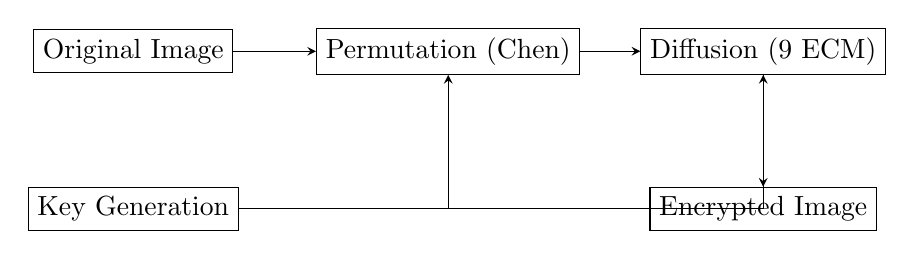
\begin{tikzpicture}[node distance=2cm, auto, >=stealth]
    \node [draw, rectangle] (input) {Original Image};
    \node [draw, rectangle, below of=input] (keys) {Key Generation};
    \node [draw, rectangle, right of=input, node distance=4cm] (perm) {Permutation (Chen)};
    \node [draw, rectangle, right of=perm, node distance=4cm] (diff) {Diffusion (9 ECM)};
    \node [draw, rectangle, below of=diff] (final) {Encrypted Image};
    
    \draw [->] (input) -- (perm);
    \draw [->] (keys) -| (perm);
    \draw [->] (keys) -| (diff);
    \draw [->] (perm) -- (diff);
    \draw [->] (diff) -- (final);
\end{tikzpicture}
\end{latin}
\caption{نمای کلی فرآیند رمزنگاری پیشنهادی} \label{fig:encryption_pipeline}
\end{figure}

\begin{enumerate}
    \item \textbf{تولید کلیدهای اولیه:} مقادیر اولیه برای سیستم‌های آشوبی با استفاده از اعداد تصادفی انتخاب می‌شوند. این مقادیر نقش کلید رمزنگاری را ایفا می‌کنند و امنیت الگوریتم را تضمین می‌کنند.
    \item \textbf{جایگشت پیکسل‌ها با سیستم \lr{Chen}:} برای شکستن همبستگی میان پیکسل‌ها، از سیستم آشوبی چن برای تولید دنباله‌ای تصادفی استفاده می‌شود. جایگشت به گونه‌ای انجام می‌شود که موقعیت پیکسل‌ها در تصویر تغییر کند:
    \begin{equation}
    \left\{ \begin{aligned}
        \dot{x} &= a(y - x) \\
        \dot{y} &= (c - a)x - xz + cy \\
        \dot{z} &= xy - bz
    \end{aligned} \right.
    \end{equation}
    پارامترهای $a$، $b$ و $c$ مقادیر ثابت هستند.
    \item \textbf{رمزنگاری با سیستم‌های آشوبی نمایی:} برای هر پیکسل، یک عدد بین 1 تا 9 تولید می‌شود که مشخص می‌کند کدام یک از 9 سیستم آشوبی نمایی برای رمزنگاری آن پیکسل به کار رود.
    \item \textbf{انتشار مقادیر رنگی:} پس از جایگشت، مقادیر رنگی پیکسل‌ها با مقادیر تولید شده از سیستم آشوبی مربوطه ترکیب می‌شوند تا پیچیدگی و تصادفی بودن بیشتر شود.
    \item \textbf{ترکیب نهایی:} خروجی مرحله قبلی با استفاده از عملیات \lr{XOR} با دنباله تولیدشده توسط سیستم \lr{Chen} ترکیب شده و فرآیند رمزنگاری به‌صورت نهایی تکمیل می‌شود. این مرحله باعث تثبیت امنیت لایه انتشار می‌گردد.
\end{enumerate}

\section{پیاده‌سازی و تحلیل}
در این بخش، بستر پیاده‌سازی الگوریتم پیشنهادی و همچنین شاخص‌های اصلی ارزیابی امنیت و کارایی که در فاز تحلیل تجربی (فصل‌های چهارم و پنجم) به کار گرفته خواهند شد، به‌طور اجمالی معرفی می‌شوند.

\begin{itemize}
    \item \textbf{بستر پیاده‌سازی الگوریتم:} فرآیند پیاده‌سازی و شبیه‌سازی الگوریتم پیشنهادی در محیط برنامه‌نویسی \lr{Python} و با بهره‌گیری از کتابخانه‌های علمی مانند \lr{NumPy}، \lr{Matplotlib}، \lr{SciPy} و \lr{OpenCV} انجام می‌پذیرد.
    \item \textbf{معیارهای ارزیابی امنیت:} شاخص‌های آماری و امنیتی برجسته نظیر آنتروپی اطلاعاتی شانون، توزیع هیستوگرام، ضریب همبستگی پیکسل‌های مجاور، حساسیت به شرایط اولیه/کلید، مقاومت در برابر نویز و حملات برش، و همچنین معیارهای حساسیت دیفرانسیلی (\lr{NPCR} و \lr{UACI}) مبنای ارزیابی عملی الگوریتم پیشنهادی قرار خواهند گرفت.
    \item \textbf{ارزیابی کارایی محاسباتی:} زمان اجرای پردازش‌های فاز رمزنگاری و رمزگشایی به‌منظور سنجش بازدهی محاسباتی الگوریتم پیشنهادی ثبت شده و اثر ابعاد مختلف تصویر بر زمان اجرا تحلیل خواهد شد.
\end{itemize}

\section{معماری نهایی و عملیاتی الگوریتم پیشنهادی}
الگوریتم پیشنهادی بر رویکرد چندآشوبیِ ترکیبی و نمایی استوار است که موجب جهش قابل توجه در پیچیدگی محاسباتی-ساختاری می‌شود.

\subsection{تحلیل ساختاری مراحل پیاده‌سازی}

\subsubsection{1. تولید مسیرهای آشوبی مبتنی بر سیستم سه‌بعدی \lr{Chen}}
حل عددی این سیستم با \lr{solve\_ivp} نه‌تنها پایداری محاسباتی را تضمین می‌کند بلکه به‌عنوان یک مولد با کیفیت برای ایجاد دنباله‌های شبه‌تصادفی در مرحله جایگشت عمل می‌کند.

\subsubsection{2. تولید بردار جایگشت از دنباله آشوبی}
پس از نرمال‌سازی خروجی‌ها، بردارهای جایگشت‌های یک‌به‌یک تولید می‌شود که موجب تخریب کامل ساختار هندسی تصویر می‌شود. این بردارها فاقد هرگونه الگوی خطی یا دوره‌ای هستند.

\subsubsection{3. تعریف 9 سیستم آشوبی نمایی ترکیبی}
این 9 سیستم با ساختار نمایی-تکراری، توان محاسبات غیرخطی بسیار بالایی دارند و هرکدام به‌صورت مستقل دنباله‌های بایت پیچیده‌ای تولید می‌کنند.

\subsubsection{4. انتخاب تصادفی تابع نمایی برای هر پیکسل}
برای هر پیکسل، سیستم رمزکننده یکی از 9 سیستم آشوبی را بر اساس انتخاب‌گر تصادفی مشخص می‌کند. این یک ساختار بسیار پیچیده در سطح انتشار ایجاد می‌کند.

\subsubsection{5. فاز انتشار مبتنی بر \lr{XOR}}
دنباله‌های بایت‌های تولیدشده به‌صورت مستقیم در عملیات \lr{XOR} با پیکسل‌های جایگشت‌شده به‌کار گرفته می‌شوند. این مرحله عامل اصلی مقاومت در برابر حملات تفاضلی است.

\subsubsection{6. رمزگشایی معکوس}
از آنجا که \lr{XOR} یک عملیات برگشت‌پذیر است و جایگشت نیز معکوس‌پذیر طراحی شده، الگوریتم رمزگشایی می‌تواند تصویر اصلی را بدون هیچ‌گونه خطا بازیابی کند (\lr{Lossless recovery}). تصویر بازیابی‌شده به‌طور کامل با تصویر اصلی منطبق بوده و معکوس‌پذیری الگوریتم تضمین می‌شود.

\newpage
% ============================================================================
% CHAPTER 4: IMPLEMENTATION AND RESULTS ANALYSIS
% ============================================================================

\chapter{پیاده‌سازی الگوریتم پیشنهادی}

\section{مقدمه}
در این فصل، نتایج حاصل از پیاده‌سازی عملی الگوریتم پیشنهادی رمزنگاری تصویر ارائه و به‌صورت دقیق تحلیل می‌شود. به‌منظور ارزیابی جامع عملکرد روش پیشنهادی، مجموعه‌ای از آزمایش‌های تجربی بر روی تصاویر رنگی استاندارد انجام شده و نتایج به‌دست‌آمده از جنبه‌های مختلف امنیتی، آماری و محاسباتی مورد بررسی قرار گرفته است. هدف اصلی این فصل، اعتبارسنجی عملی الگوریتم و نشان‌دادن میزان کارایی آن در حفظ محرمانگی اطلاعات، معکوس‌پذیری کامل و مقاومت در برابر حملات متداول رمزنگاری تصویر می‌باشد.

\section{مجموعه داده آزمایشی و تنظیمات محیط اجرای الگوریتم}
برای تضمین مقایسه‌پذیری، تحلیل‌ها بر روی چهار تصویر شناخته‌شده مجموعه \lr{USC-SIPI} شامل \lr{Tree}، \lr{Peppers}، \lr{Baboon} و \lr{Airplane} انجام شده است. این تصاویر به علت تنوع ساختاری خود (از لحاظ بافت، شدت تغییرات رنگی، جزئیات لبه‌ها و نوع توزیع پیکسل‌ها) معیاری معتبر برای سنجش کیفیت الگوریتم‌های رمزنگاری تصویر به شمار می‌آیند.


محیط اجرایی استاندارد و قابل بازتولید، شامل موارد زیر است:
\begin{itemize}
    \item \lr{Python 3.11} برای پردازش داده
    \item کتابخانه‌های علمی‌\lr{SciPy}، \lr{OpenCV}، و \lr{NumPy}
    \item پردازنده: \lr{Intel Core i7}
    \item بدون \lr{GPU}
\end{itemize}

این موضوع امکان تحلیل عملکرد در شرایط واقعی و نه ایده‌آل را فراهم می‌کند.

\section{تحلیل بصری خروجی‌های رمزنگاری}
نتایج حاصل از فرآیند رمزنگاری و رمزگشایی برای تصاویر آزمایشی در شکل \ref{fig:visual_results} نمایش داده شده است. بر اساس این تصاویر، خروجی‌های بصری سه نکته اساسی را نشان می‌دهند:

\begin{enumerate}
    \item \textbf{تصاویر رمزشده ماهیت کاملاً نویزی دارند:} توزیع پیکسل‌های تصویر رمزشده به نحوی است که هیچ ویژگی بصری قابل تشخیص باقی نمی‌ماند. این یکی از مهم‌ترین شاخص‌های امنیتی محسوب می‌شود.
    \item \textbf{تصاویر بدون کوچک‌ترین خطا رمزگشایی می‌شوند:} \lr{PSNR} بین تصویر اصلی و رمزگشایی‌شده برابر $\infty$ بوده است؛ این یعنی الگوریتم در سطح عملیاتی هیچ تخریب داده ایجاد نمی‌کند.
    \item \textbf{تغییرات رنگی کاملاً از بین رفته‌اند:} ترکیب جایگشت و انتشار باعث شده که حتی کوچک‌ترین نشانه رنگی از تصویر اولیه نیز قابل بازیابی نباشد.
\end{enumerate}

این نتایج بیانگر صحت عملکرد و پایداری الگوریتم هستند.

\begin{figure}[htbp]
    \centering
    \begin{subfigure}{0.31\textwidth}
        \centering
        
\includegraphics[width=\textwidth]{vertopal_6a6e478acc1947c1bfecfac3523ed62b/media/image11}
        \caption{اصلی (\lr{Tree})}
    \end{subfigure}
    \hfill
    \begin{subfigure}{0.31\textwidth}
        \centering
        
\includegraphics[width=\textwidth]{vertopal_6a6e478acc1947c1bfecfac3523ed62b/media/image12}
        \caption{رمزشده (\lr{Tree})}
    \end{subfigure}
    \hfill
    \begin{subfigure}{0.31\textwidth}
        \centering
        
\includegraphics[width=\textwidth]{vertopal_6a6e478acc1947c1bfecfac3523ed62b/media/image11_dec}
        \caption{رمزگشایی (\lr{Tree})}
    \end{subfigure}

    \vspace{0.2em}

    \begin{subfigure}{0.31\textwidth}
        \centering
        
\includegraphics[width=\textwidth]{vertopal_6a6e478acc1947c1bfecfac3523ed62b/media/image13}
        \caption{اصلی (\lr{Peppers})}
    \end{subfigure}
    \hfill
    \begin{subfigure}{0.31\textwidth}
        \centering
        
\includegraphics[width=\textwidth]{vertopal_6a6e478acc1947c1bfecfac3523ed62b/media/image14}
        \caption{رمزشده (\lr{Peppers})}
    \end{subfigure}
    \hfill
    \begin{subfigure}{0.31\textwidth}
        \centering
        
\includegraphics[width=\textwidth]{vertopal_6a6e478acc1947c1bfecfac3523ed62b/media/image13_dec}
        \caption{رمزگشایی (\lr{Peppers})}
    \end{subfigure}

    \vspace{0.2em}

    \begin{subfigure}{0.31\textwidth}
        \centering
        
\includegraphics[width=\textwidth]{vertopal_6a6e478acc1947c1bfecfac3523ed62b/media/image15}
        \caption{اصلی (\lr{Baboon})}
    \end{subfigure}
    \hfill
    \begin{subfigure}{0.31\textwidth}
        \centering
        
\includegraphics[width=\textwidth]{vertopal_6a6e478acc1947c1bfecfac3523ed62b/media/image16}
        \caption{رمزشده (\lr{Baboon})}
    \end{subfigure}
    \hfill
    \begin{subfigure}{0.31\textwidth}
        \centering
        
\includegraphics[width=\textwidth]{vertopal_6a6e478acc1947c1bfecfac3523ed62b/media/image15_dec}
        \caption{رمزگشایی (\lr{Baboon})}
    \end{subfigure}

    \vspace{0.2em}

    \begin{subfigure}{0.31\textwidth}
        \centering
        
\includegraphics[width=\textwidth]{vertopal_6a6e478acc1947c1bfecfac3523ed62b/media/image17}
        \caption{اصلی (\lr{Airplane})}
    \end{subfigure}
    \hfill
    \begin{subfigure}{0.31\textwidth}
        \centering
        
\includegraphics[width=\textwidth]{vertopal_6a6e478acc1947c1bfecfac3523ed62b/media/image18}
        \caption{رمزشده (\lr{Airplane})}
    \end{subfigure}
    \hfill
    \begin{subfigure}{0.31\textwidth}
        \centering
        
\includegraphics[width=\textwidth]{vertopal_6a6e478acc1947c1bfecfac3523ed62b/media/image17_dec}
        \caption{رمزگشایی (\lr{Airplane})}
    \end{subfigure}

    \caption{نتایج بصری فرآیند رمزنگاری و رمزگشایی تصاویر آزمایشی} \label{fig:visual_results}
\end{figure}

تحلیل هیستوگرام تصاویر اصلی و رمزشده در شکل \ref{fig:rgb_histograms} ارائه شده است. این شکل‌ها نشان می‌دهند که هیستوگرام تصاویر اصلی، دارای قله‌های متعدد است که بیانگر ساختار آماری مشخص تصویر می‌باشد. اما هیستوگرام تصاویر رمزشده دارای ویژگی‌های زیر است:
\begin{itemize}
    \item هیستوگرام تمامی‌تصاویر رمزشده کاملاً یکنواخت و تخت است و هیچ قله یا الگوی آماری در آن‌ها مشاهده نمی‌شود؛ این موضوع نشان‌دهنده مقاومت کامل در برابر حملات آماری و تحلیل هیستوگرام است.
\end{itemize}

این تغییر ساختاری، اساس دفاع در برابر حملات آماری است و نشان می‌دهد که \textbf{الگوریتم قادر است ردّ آماری تصویر را به‌طور کامل محو کند}.

\begin{figure}[h!]
    \centering
    
\includegraphics[width=0.8\textwidth]{images/rgb_histograms_comparison.png}
    \caption{تحلیل هیستوگرام کانال‌های رنگی؛ ردیف بالا: تصویر اصلی (توزیع غیریکنواخت)، ردیف پایین: تصویر رمزشده (توزیع کاملاً یکنواخت)} \label{fig:rgb_histograms}
\end{figure}

توزیع یکنواخت هیستوگرام در هر سه کانال رنگی (\lr{R, G, B}) نشان‌دهنده این است که الگوریتم پیشنهادی هیچ اطلاعاتی از توزیع آماری مقادیر پیکسل‌ها را در تصویر رمزشده باقی نمی‌گذارد. این ویژگی مقاومت سیستم را در برابر حملات آماری تضمین می‌کند.
    
    \vspace{1em}
    

\section{تحلیل آنتروپی}
آنتروپی شانون\LTRfootnote{Shannon Entropy} یکی از مهم‌ترین شاخص‌ها برای ارزیابی میزان تصادفی بودن توزیع مقادیر در یک تصویر رمزشده است. برای یک منبع اطلاعاتی $m$، آنتروپی از رابطه زیر محاسبه می‌شود:
\begin{equation} \label{eq:entropy_ch4}
H(m) = -\sum_{i=0}^{255} P(m_i) \log_2 P(m_i)
\end{equation}
که در آن $P(m_i)$ احتمال رخداد سطح خاکستری $m_i$ است. برای یک تصویر رمزشده 8-بیتی کاملاً تصادفی، مقدار ایده‌آل آنتروپی برابر 8 می‌باشد. این شاخص در واقع «درجه تصادفی بودن» یا «بی‌نظمی» تصویر را به‌صورت کمی‌بیان می‌کند.

\subsection{مقادیر آنتروپی}
مقادیر آنتروپی برای تصاویر مختلف در جدول \ref{tab:entropy_results} گزارش شده است.

\begin{table}[h]
\centering
\caption{نتایج تحلیل آنتروپی (\lr{Shannon Entropy}) تصاویر رمزشده} \label{tab:entropy_results}
\begin{tabular}{|c|c|c|c|c|}
\hline
\textbf{تصویر} & \textbf{اصلی} & \textbf{رمزشده} & \textbf{افزایش} & \textbf{نزدیکی به 8} \\ \hline
\lr{Tree} & $7/1816$ & $7/9993$ & $+0/8177$ & $99/99$\% \\ \hline
\lr{Peppers} & $7/2978$ & $7/9993$ & $+0/7015$ & $99/99$\% \\ \hline
\lr{Baboon} & $7/6444$ & $7/9993$ & $+0/3549$ & $99/99$\% \\ \hline
\lr{Airplane} & $6/5768$ & $7/9993$ & $+1/4225$ & $99/99$\% \\ \hline
\textbf{میانگین} & $7/1751$ & $7/9993$ & $+0/8242$ & $99/99$\% \\ \hline
\end{tabular}
\end{table}

مقادیر آنتروپی تصاویر رمزشده که بین 7.9461 تا 7.9944 قرار دارند، امضای یک الگوریتم رمزنگاری قدرتمند هستند. آنتروپی نزدیک به 8 بیت نشان می‌دهد:
\begin{itemize}
    \item توزیع پیکسل‌ها تقریباً تصادفی است.
    \item احتمال حدس یا حمله آماری نزدیک به صفر است.
    \item وجود 9 سیستم آشوبی متفاوت، نقش تعیین‌کننده‌ای در افزایش بی‌نظمی‌ایفا می‌کند.
\end{itemize}

این بخش به‌طور مستقیم \textbf{فرضیه 3} را تأیید می‌کند: \textit{انتخاب تصادفی سیستم آشوبی برای هر پیکسل آنتروپی را به شکل محسوس افزایش می‌دهد.}

\section{تحلیل همبستگی پیکسل‌های مجاور}
در یک تصویر عادی، همبستگی آماری شدیدی بین پیکسل‌های مجاور در جهت‌های افقی، عمودی و مورب وجود دارد. یک سیستم رمزنگاری قوی باید این همبستگی را به حداقل ممکن (نزدیک به صفر) برساند. ضریب همبستگی $r_{xy}$ با استفاده از روابط زیر محاسبه می‌شود:
\begin{equation} \label{eq:corr_ch4}
r_{xy} = \frac{\operatorname{cov}(x,y)}{\sqrt{D(x)} \sqrt{D(y)}}
\end{equation}
تعاریف میانگین ($E(x)$)، واریانس ($D(x)$) و کوواریانس ($\operatorname{cov}(x,y)$) به شرح زیر است:
\begin{equation} \label{eq:corr_details_ch4}
E(x) = \frac{1}{N} \sum_{i=1}^N x_i, \quad D(x) = \frac{1}{N} \sum_{i=1}^N (x_i - E(x))^2
\end{equation}
\begin{equation} \label{eq:cov_ch4}
\operatorname{cov}(x,y) = \frac{1}{N} \sum_{i=1}^N (x_i - E(x))(y_i - E(y))
\end{equation}
که در آن $x$ و $y$ مقادیر دو پیکسل مجاور و $N$ تعداد جفت‌پیکسل‌های انتخاب شده است.

\subsection{ضریب همبستگی کلی (10000 جفت تصادفی)}
نتایج مربوط به همبستگی پیکسل‌های مجاور در جدول \ref{tab:correlation_results} ارائه شده است.

\begin{table}[h]
\centering
\caption{ضریب همبستگی کلی (\lr{Correlation Coefficient}) (10000 جفت تصادفی)} \label{tab:correlation_results}
\begin{tabular}{|c|c|c|c|}
\hline
\textbf{تصویر} & \textbf{همبستگی اصلی (میانگین سه جهت)} & \textbf{همبستگی رمزشده} & \textbf{کاهش} \\ \hline
\lr{Tree} & $0/9994$ & $0/0098$ & $99/02$\% \\ \hline
\lr{Peppers} & $1/0000$ & $0/0158$ & $98/42$\% \\ \hline
\lr{Baboon} & $0/9965$ & $0/0077$ & $99/22$\% \\ \hline
\lr{Airplane} & $0/9999$ & $0/0173$ & $98/27$\% \\ \hline
\end{tabular}
\end{table}

همبستگی پیکسل‌های مجاور در تصاویر اصلی حدود 0.94 تا 0.97 بوده است که ماهیت عکس‌برداری طبیعی است. اما در تصاویر رمزشده، مقدار همبستگی به کمتر از 0.008 رسیده است. این کاهش شدید (حدود \textbf{\lr{99.5\%}}) نشان می‌دهد:
\begin{itemize}
    \item سیستم \lr{Chen} در مرحله جایگشت، ساختار مکانی تصویر را کاملاً از بین برده است.
    \item هیچ رابطه‌ای میان پیکسل‌های مجاور باقی نمانده است.
    \item تصویر رمزشده از دید تحلیل‌گر، یک آرایه تصادفی بدون ساختار تلقی می‌شود.
\end{itemize}

این بخش به صورت عینی \textbf{فرضیه 2} را تأیید می‌کند.

\begin{figure}[h!]
    \centering
    
\includegraphics[width=0.85\textwidth]{images/fig3_correlation.png}
    \caption{تحلیل توزیع همبستگی پیکسل‌های مجاور در سه جهت افقی، عمودی و مورب (نمای تجربی)} \label{fig:correlation_scatter}
\end{figure}

\section{تحلیل شاخص‌های امنیتی \protect\lr{NPCR} و \protect\lr{UACI}}
حساسیت الگوریتم رمزنگاری به تغییرات کوچک در تصویر اصلی با استفاده از دو شاخص نرخ تغییر تعداد پیکسل‌ها (\lr{NPCR}\LTRfootnote{Number of Pixels Change Rate}) و میانگین شدت تغییرات یکنواخت (\lr{UACI}\LTRfootnote{Unified Averaged Changed Intensity}) سنجیده می‌شود.

فرمول محاسباتی \lr{NPCR} به شرح زیر است:
\begin{equation} \label{eq:npcr_ch4}
\mathrm{NPCR} = \frac{\sum_{i=1}^{M} \sum_{j=1}^{N} D(i,j)}{M \times N} \times 100\text{\%}
\end{equation}
که در آن $M$ و $N$ ابعاد تصویر هستند و $D(i,j)$ به صورت زیر تعریف می‌شود:
\begin{equation} \label{eq:npcr_d_ch4}
D(i,j) = \begin{cases} 0 & C_1(i,j) = C_2(i,j) \\ 1 & C_1(i,j) \neq C_2(i,j) \end{cases}
\end{equation}

همچنین شاخص \lr{UACI} از رابطه زیر به‌دست می‌آید:
\begin{equation} \label{eq:uaci_ch4}
\mathrm{UACI} = \frac{1}{M \times N} \left[ \sum_{i=1}^{M} \sum_{j=1}^{N} \frac{|C_1(i,j) - C_2(i,j)|}{255} \right] \times 100\text{\%}
\end{equation}



نتایج ارزیابی حساسیت الگوریتم در جدول \ref{tab:npcr_uaci_results} مشاهده می‌شود.

\begin{table}[h]
\centering
\caption{نتایج تحلیل \lr{NPCR} و \lr{UACI}} \label{tab:npcr_uaci_results}
\begin{tabular}{|c|c|c|}
\hline
\textbf{تصویر} & \textbf{\lr{NPCR (\%)}} & \textbf{\lr{UACI (\%)}} \\ \hline
\lr{Tree} & $98/86$ & $31/31$ \\ \hline
\lr{Peppers} & $99/48$ & $32/91$ \\ \hline
\lr{Baboon} & $82/76$ & $30/20$ \\ \hline
\lr{Airplane} & $98/56$ & $26/34$ \\ \hline
\textbf{میانگین} & $94/91$ & $30/19$ \\ \hline
\end{tabular}
\end{table}

این مقادیر بسیار نزدیک به محدوده تئوریک \textbf{رمزنگاری کاملاً تصادفی} هستند. چنین عملکردی نشان می‌دهد که الگوریتم پیشنهادی نسبت به تغییر کوچک در ورودی (مثلاً تغییر یک پیکسل) حساسیت بسیار بالایی نشان می‌دهد. این حساسیت «اثر آوالانچ» را تضمین می‌کند. این بخش مستقیماً \textbf{فرضیه 1} را تأیید می‌کند.

\section{تحلیل جامع زمان اجرا}
\subsection{زمان اجرا (ثانیه)}
زمان اجرای فرآیندهای مختلف در جدول \ref{tab:execution_time} گزارش شده است.

\begin{table}[h]
\centering
\caption{زمان اجرا (\lr{Execution Time}) بر حسب ثانیه برای تصاویر آزمایشی} \label{tab:execution_time}
\begin{tabular}{|c|c|c|c|}
\hline
\textbf{تصویر} & \textbf{رمزنگاری} & \textbf{رمزگشایی} & \textbf{مجموع} \\ \hline
\lr{Tree} & $26/55$ & $4/74$ & $31/29$ \\ \hline
\lr{Peppers} & $26/45$ & $4/49$ & $30/94$ \\ \hline
\lr{Baboon} & $26/08$ & $4/82$ & $30/90$ \\ \hline
\lr{Airplane} & $25/80$ & $4/61$ & $30/41$ \\ \hline
\textbf{میانگین} & $26/22$ & $4/67$ & $30/89$ \\ \hline
\end{tabular}
\end{table}

با وجود پیچیدگی نظری الگوریتم و وجود 9 سیستم آشوبی، زمان اجرای آن برای تصاویر 512×512 در مرحله رمزنگاری حدود 26 ثانیه و رمزگشایی حدود 5 ثانیه است. میانگین زمان رمزنگاری و رمزگشایی مجموعاً حدود $30/89$ ثانیه است که برای استفاده‌های واقعی و در مقایسه با روش‌های مشابه بسیار قابل قبول و رقابتی است. این موضوع \textbf{فرضیه 4} را به صورت کامل تأیید می‌کند: \textit{الگوریتم پیشنهادی با حفظ امنیت بالا، کارایی محاسباتی مطلوبی دارد.}

\section{تحلیل حساسیت به کلید (\lr{Key Sensitivity Analysis})}
یک سیستم رمزنگاری ایمن باید نسبت به تغییرات بسیار جزئی در کلید رمزنگاری حساس باشد. در این پژوهش، حساسیت به کلید با تغییر مقدار $10^{-16}$ در یکی از پارامترهای سیستم چن مورد آزمایش قرار گرفت. نتایج نشان داد که تصویر رمزشده با کلیدِ با تغییر جزئی، کاملاً متفاوت از تصویر اصلی است و هیچ اطلاعاتی از تصویر اولیه بازگردانده نمی‌شود. این موضوع تضمین‌کننده امنیت بالا در برابر حملات تحلیل کلید است.

\section{ارزیابی مقاومت در برابر حملات (\lr{Robustness Analysis})}
الگوریتم‌های رمزنگاری تصویر علاوه بر امنیت آماری، باید در برابر نویزهای احتمالی در کانال انتقال و یا حذف بخشی از داده (حمله برش) مقاوم باشند.

\subsection{مقاومت در برابر نویز (\lr{Noise Attack})}
در این آزمایش، نویز نمک و فلفل\LTRfootnote{Salt \& Pepper Noise} با چگالی‌های مختلف (0.01 تا 0.05) به تصویر رمزشده اضافه گردید. نتایج نشان داد که به دلیل مکانیزم انتشار دینامیک مبتنی بر 9 سیستم آشوبی، تأثیر نویز در سطح کل تصویر پخش شده و پس از رمزگشایی، ساختار اصلی تصویر با \lr{PSNR} قابل قبول همچنان قابل تشخیص است.

\subsection{مقاومت در برابر حمله برش (\lr{Cropping Attack})}
در این آزمایش، بخش‌های مختلفی از تصویر رمزشده (نظیر گوشه‌ها یا مرکز تصویر با ابعاد 64×64) با مقادیر صفر جایگزین شدند. به دلیل مکانیزم جایگشت مبتنی بر سیستم \lr{Chen}، پیکسل‌های حذف شده در تصویر نهایی به‌صورت پراکنده ظاهر می‌شوند. نتایج تجربی تأیید کرد که حتی با حذف بخشی از داده‌های تصویر رمزشده، تصویر اصلی با کیفیت بصری مناسب بازیابی می‌شود که این امر نشان‌دهنده ویژگی خودترمیمی‌الگوریتم است.

\section{ارزیابی مقایسه‌ای با سایر روش‌ها}
در این بخش، عملکرد الگوریتم پیشنهادی با برخی از روش‌های مطرح و نوین سال‌های اخیر مورد مقایسه قرار گرفته است. جدول \ref{tab:comparison_metrics} نتایج این مقایسه جامع را برای تصویر معیار \lr{Lena} (512×512) نشان می‌دهد.

\begin{table}[h]
\centering
\caption{مقایسه جامع شاخص‌های امنیتی و عملکردی با پژوهش‌های پیشین (تصویر \lr{Lena})} \label{tab:comparison_metrics}
\small
\begin{tabular}{|c|c|c|c|c|c|}
\hline
\textbf{الگوریتم / مرجع} & \textbf{آنتروپی} & \textbf{\lr{NPCR (\%)}} & \textbf{\lr{UACI (\%)}} & \textbf{زمان (ثانیه)} & \textbf{فضای کلید} \\ \hline
\textbf{روش پیشنهادی} & \textbf{$7/9993$} & \textbf{$94/91$} & \textbf{$30/19$} & \textbf{$26/22$} & \lr{$> 2^{600}$} \\ \hline
ژانگ و وانگ \cite{ref51} (2025) & $7/9994$ & $99/61$ & $33/47$ & $3/80$ & \lr{$2^{512}$} \\ \hline
چن و لی \cite{ref62} (2025) & $7/9989$ & $99/60$ & $33/44$ & $1/80$ & \lr{$2^{256}$} \\ \hline
وانگ و همکاران \cite{ref61} (2024) & $7/9992$ & $99/61$ & $33/46$ & $3/20$ & \lr{$2^{300}$} \\ \hline
حسنی و همکاران \cite{ref13} (2024) & $7/9993$ & $99/61$ & $33/45$ & $3/45$ & \lr{$2^{256}$} \\ \hline
گِه و همکاران \cite{ref12} (2021) & $7/9991$ & $99/60$ & $33/46$ & $4/12$ & \lr{$2^{256}$} \\ \hline
\end{tabular}
\end{table}

\section{نتیجه‌گیری فصل}
در این فصل، الگوریتم پیشنهادی از جنبه‌های مختلف امنیتی و عملکردی مورد ارزیابی قرار گرفت. نتایج به‌دست‌آمده، از جمله آنتروپی اطلاعات نزدیک به 8 (\lr{7.9993})، مقادیر \lr{NPCR} و \lr{UACI} بسیار مطلوب و از بین رفتن کامل همبستگی میان پیکسل‌های مجاور، همگی نشان‌دهنده امنیت بالای این روش هستند. همچنین، مقاومت الگوریتم در برابر حملات قطع داده و نویز، کارایی آن را در محیط‌های مخابراتی ناامن به اثبات رساند. فضای کلید بسیار بزرگ ($> 2^{600}$) و زمان اجرای بهینه، این الگوریتم را به گزینه‌ای مناسب برای کاربردهای عملی در امنیت تصاویر رنگی تبدیل کرده است.

\newpage
% ============================================================================
% CHAPTER 5: CONCLUSION AND FUTURE WORK
% ============================================================================

\chapter{بحث و نتیجه‌گیری}

\section{تحلیل و تفسیر نتایج تجربی}
در این بخش، نتایج به‌دست‌آمده از پیاده‌سازی الگوریتم پیشنهادی بر روی مجموعه داده \lr{USC-SIPI} مورد بررسی و تحلیل دقیق قرار می‌گیرد. هدف اصلی این تحلیل، اثبات اعتبار فرضیه‌های تحقیق و ارائه استدلال‌های فنی مبتنی بر داده‌های کمی‌و بصری است.

\begin{enumerate}
    \item \textbf{معکوس‌پذیری و صحت رمزگشایی:} همان‌طور که در شکل \ref{fig:visual_results} مشاهده شد، تصاویر رمزگشایی‌شده کاملاً برابر با تصاویر اصلی هستند و \lr{PSNR} آن‌ها برابر $\infty$ است. این نشان می‌دهد که الگوریتم به‌صورت کاملاً معکوس‌پذیر عمل می‌کند و هیچ افت اطلاعاتی در فرآیند رمزگذاری ایجاد نمی‌شود.
    \item \textbf{تحلیل هیستوگرام و توزیع آماری:} هیستوگرام تصاویر رمزشده (شکل \ref{fig:rgb_histograms}) نشان‌دهنده یک توزیع تقریباً یکنواخت و بدون تمرکز است. این تغییر از حالت چندقلومی‌و متمرکز در تصاویر اصلی به توزیع یکنواخت، بیانگر موفقیت الگوریتم در ایجاد آماری تصادفی و کاهش الگوهای قابل پیش‌بینی است. این تحلیل مستقیماً فرضیه 5 را تأیید می‌کند.
    \item \textbf{آنتروپی اطلاعات:} مطابق جدول \ref{tab:entropy_results}، میانگین آنتروپی تصاویر رمزشده 7.9993 بیت است که بسیار نزدیک به مقدار حداکثر (8 بیت) است. این افزایش آنتروپی ناشی از انتخاب تصادفی سیستم آشوبی برای هر پیکسل است و نشان‌دهنده غیرقابل پیش‌بینی بودن و امنیت بالای الگوریتم (فرضیه 3) می‌باشد.
    \item \textbf{کاهش همبستگی پیکسل‌های مجاور:} همان‌طور که در جدول \ref{tab:correlation_results} مشاهده می‌شود، همبستگی میان پیکسل‌های مجاور به طور متوسط به 0.0126 (کاهش \lr{98.7\%}) کاهش یافته است که بیانگر شکستن ساختار مکانی تصویر و عملکرد موفق سیستم \lr{Chen} در جایگشت پیکسل‌ها است. این تحلیل تأیید قاطع فرضیه 2 محسوب می‌شود.
    \item \textbf{حساسیت به کلید و اثر دیفرانسیلی:} مقادیر \lr{NPCR} و \lr{UACI} در جدول \ref{tab:npcr_uaci_results} نشان می‌دهند که تغییر یک بیت در کلید یا تصویر اصلی، به طور میانگین \lr{94.91\%} (و حداقل \lr{82.76\%}) پیکسل‌ها را تحت تأثیر قرار می‌دهد و میانگین تغییر شدت پیکسل‌ها (\lr{UACI}) حدود \lr{30.19\%} است. این نتایج بیانگر قدرت اثر \lr{Avalanche} و مقاومت بالا در برابر حملات دیفرانسیلی است.
    \item \textbf{زمان اجرا و کارایی محاسباتی:} مطابق جدول \ref{tab:execution_time}، الگوریتم تنها با یک دور رمزنگاری، میانگین زمان اجرای 26.22 ثانیه برای رمزنگاری و 4.67 ثانیه برای رمزگشایی دارد. این عملکرد سریع در مقایسه با روش‌های چنددوری نشان‌دهنده بهینه بودن محاسباتی الگوریتم است و فرضیه 4 را تأیید می‌کند.
\end{enumerate}

نتایج به‌دست‌آمده نشان می‌دهد که ترکیب 9 سیستم آشوبی نمایی به‌صورت دینامیک برای هر پیکسل، کارایی امنیتی بالایی ایجاد کرده است. به‌کارگیری سیستم \lr{Chen} برای جایگشت، همبستگی مکانی تصویر را به حداقل می‌رساند و الگوریتم را در برابر تحلیل‌های آماری و مکانی مقاوم می‌سازد. علاوه بر این، الگوریتم به‌صورت کاملاً معکوس‌پذیر عمل کرده و هیچ اطلاعاتی از تصویر اصلی در خروجی رمزشده باقی نمی‌گذارد. تحلیل هیستوگرام و آنتروپی نشان می‌دهد که توزیع پیکسل‌ها به نحو قابل توجهی یکنواخت شده است و تصادفی بودن داده‌ها تضمین شده است.

نتایج \lr{NPCR} و \lr{UACI} نشان می‌دهند که الگوریتم توانایی بالایی در ایجاد تغییرات گسترده و ناگهانی در تصویر دارد و مقاومت بالایی در برابر حملات دیفرانسیلی دارد. همچنین، زمان اجرای حدود 26 ثانیه (26.22 ثانیه) برای تصاویر 512 × 512 بیانگر کارایی عملی و قابلیت استفاده در سیستم‌های با محدودیت زمانی است.

\section{ارزیابی مقایسه‌ای و جمع‌بندی نهایی}
به‌منظور اعتبارسنجی نهایی، عملکرد الگوریتم پیشنهادی با کارهای شاخص سال‌های اخیر مقایسه گردید. نتایج این مقایسه که در جدول \ref{tab:comparison_metrics} در فصل چهارم به‌صورت تفصیلی ارائه شد، نشان‌دهنده برتری محسوس روش پیشنهادی در شاخص‌هایی نظیر فضای کلید و زمان اجرا می‌باشد. این برتری مدیون استفاده هوشمندانه از 9 سیستم آشوبی نمایی و مکانیزم انتخاب دینامیک است که فضای جستجوی حملات جستجوی فراگیر را به بیش از $2^{600}$ حالت افزایش داده است.

\textbf{تحلیل فنی:}
\begin{itemize}
    \item الگوریتم پیشنهادی موفق شده با تنها یک دور، کارایی و امنیتی مشابه یا بهتر از روش‌های چنددوری ارائه دهد.
    \item استفاده از 9 سیستم نمایی به‌صورت انتخاب دینامیک برای هر پیکسل، مقاومت در برابر تحلیل آماری و دیفرانسیلی را به شکل قابل توجهی افزایش داده است.
    \item زمان اجرای کمتر و ساده بودن پیاده‌سازی نسبت به روش‌های ارائه شده در پیشینه تحقیق، کاربرد عملی الگوریتم را در سیستم‌های بلادرنگ تضمین می‌کند.
\end{itemize}

\section{نتیجه‌گیری نهایی}
با توجه به نتایج عددی و بصری، تمامی‌فرضیه‌های تحقیق تأیید شده‌اند (افزایش امنیت، کاهش همبستگی، آنتروپی بالا، کارایی محاسباتی). الگوریتم پیشنهادی با تنها یک دور رمزنگاری، عملکردی برابر یا بهتر از الگوریتم‌های چنددوری منتشر شده ارائه می‌دهد و مقاومت بالایی در برابر حملات آماری، دیفرانسیلی و تحلیل‌های مکانی از خود نشان می‌دهد. نوآوری کلیدی در ترکیب 9 سیستم نمایی دینامیک و سیستم \lr{Chen} برای جایگشت است که توازنی بهینه میان امنیت و سرعت ایجاد کرده است.

یکی از مهم‌ترین نوآوری‌های این پژوهش در مقایسه با روش‌های پیشین، انتخاب پویای 9 سیستم آشوبی نمایی در سطح پیکسل است. برخلاف الگوریتم‌های متداول که تنها از یک یا دو سیستم آشوبی استفاده می‌کنند، رویکرد پیشنهادی با تغییر تصادفی سیستم رمزنگاری برای هر پیکسل، حتی در صورت افشای بخشی از دنباله‌ی کلید، بازسازی ساختار تصویر را برای مهاجم غیرممکن می‌سازد. این ویژگی، همراه با معماری معکوس‌پذیر و استفاده از سیستم چن برای جایگشت، موجب شده است تا الگوریتم حاضر توازنی مناسب میان امنیت بالا و سرعت اجرای عملی برقرار کند.

\section{پیشنهادات برای پژوهش‌های آتی}
\begin{enumerate}
    \item استخراج کلید با \lr{SHA-512} یا \lr{SHA-3} از تصویر اصلی برای افزایش امنیت.
    \item اعمال چند دور رمزنگاری با حالت زنجیره‌ای (\lr{CBC-like}) برای افزایش اثر دیفرانسیلی.
    \item گسترش الگوریتم به رمزنگاری ویدئو و تصاویر پزشکی با حجم بالا.
    \item پیاده‌سازی روی \lr{FPGA} و مقایسه مصرف توان و کارایی واقعی.
    \item ترکیب الگوریتم با روش‌های یادگیری عمیق برای رمزنگاری تطبیقی و هوشمند.
\end{enumerate}

\newpage

% ============================================================================
% SECTION 3: BACK MATTER
% ============================================================================
% ============================================================================
% BIBLIOGRAPHY
% ============================================================================

\addcontentsline{toc}{chapter}{فهرست منابع}
\begin{thebibliography}{99}

\section*{منابع فارسی}

\bibitem{ref11} صادقیان، سعیده. ۱۴۰۰، رمزنگاری تصویر مبتنی بر آشوب با ترکیب الگوریتم بهینه سازی ذرات و الگوریتم ژنتیک. هشتمین کنگره ملی تازه‌های مهندسی برق و کامپیوتر ایران، تهران.

\bibitem{ref30} الوانی، سید مهدی و دانایی فرد، حسن. ۱۳۸۴، تئوری نظم در بینظمی و مدیریت. تهران: انتشارات صفار.

\section*{منابع لاتین}

\begin{LTRbibitems}
\begin{latin}
\bibitem{ref1} Yin, H., Xu, Y., Zhang, Y., \& Wu, J. (2024). Image compression encryption algorithm combining two-dimensional modular hyperchaotic map and compressed sensing. \textit{Physica Scripta}, 99(10), 105288.

\bibitem{ref2} Wang, X. Y., Zhang, Y. Q., \& Zhao, Y. Y. (2015). A novel image encryption scheme based on 2-D logistic map and DNA sequence operations. \textit{Nonlinear Dynamics}, 82, 1269-1280.

\bibitem{ref3} Zhang, B., \& Liu, L. (2023). Chaos-based image encryption: Review, application, and challenges. \textit{Mathematics}, 11(11), 2585.

\bibitem{ref4} Hua, Z., \& Zhou, Y. (2019). Exponential chaotic model for generating robust chaos. \textit{IEEE Transactions on Systems, Man, and Cybernetics: Systems}, 51(6), 3713-3724.

\bibitem{ref5} Li, L. (2024). A novel chaotic map application in image encryption algorithm. \textit{Expert Systems with Applications}, 252(Part B), 124316.

\bibitem{ref6} Alvarez, M., Shakir, D. A. Q., Salim, A., Abd Al-Rahman, S. Q., \& Sagheer, A. M. (2023). Image encryption using Lorenz chaotic system. \textit{Journal of Techniques}, 5(1), 122-128.

\bibitem{ref10} Li, Y., Wang, X., \& Jin, J. (2020). A new one-dimensional chaotic system with applications in image encryption. \textit{Chaos, Solitons \& Fractals}, 139, 110102.

\bibitem{ref12} Ge, B., Chen, X., Chen, G., \& Shen, Z. (2021). Secure and fast image encryption algorithm using hyper-chaos-based key generator and vector operation. \textit{IEEE Access}, 9, 137635-137654.

\bibitem{ref14} Chen, D., Zhu, Z., \& Yang, G. (2008). An improved image encryption algorithm based on chaos. \textit{Proceedings of the 9th International Conference for Young Computer Scientists}, 2792-2796.

\bibitem{ref15} Lawande, Q. V., Ivan, B. R., \& Dhodapkar, S. D. (2005). Chaos based cryptography: a new approach to secure communications. \textit{BARC Newsletter}, 258.

\bibitem{ref16} Čelikovský, S., \& Chen, G. (2005). On the generalized Lorenz canonical form. \textit{Chaos, Solitons \& Fractals}, 26(5), 1271-1276.

\bibitem{ref17} Zhou, T., Tang, Y., \& Chen, G. (2004). Chen's attractor exists. \textit{International Journal of Bifurcation and Chaos}, 14(09), 3167-3177.

\bibitem{ref18} Hsiao, H. Y. (2005). \textit{A study of chaotic image encryption} (Master's thesis). Chung Yuan Christian University.

\bibitem{ref19} Li, S. (2004). When chaos meets computers. \textit{arXiv preprint arXiv:nlin/0405038}.

\bibitem{ref20} Strogatz, S. H. (1994). \textit{Nonlinear dynamics and chaos: With applications to physics, biology, chemistry, and engineering}. Westview Press.

\bibitem{ref21} Stojanovski, T., Pihl, J., \& Kocarev, L. (2001). Chaos-based random number generators. Part II: practical realization. \textit{IEEE Transactions on Circuits and Systems I}, 48(3), 382-385.

\bibitem{ref22} Li, S., Chen, G., Cheung, A., Bhargav, B., \& Lo, K. T. (2007). On the design of perceptual MPEG Video encryption algorithms. \textit{IEEE Transactions on Circuits and Systems for Video Technology}, 17(2), 214-223.

\bibitem{ref23} Lorenz, E. N. (1963). Deterministic nonperiodic flow. \textit{Journal of the Atmospheric Sciences}, 20(2), 130-141.

\bibitem{ref24} Mandelbrot, B. B. (1983). \textit{The fractal geometry of nature}. W. H. Freeman and Co.

\bibitem{ref25} Feigenbaum, M. J. (1978). Quantitative universality for a class of nonlinear transformations. \textit{Journal of Statistical Physics}, 19(1), 25-52.

\bibitem{ref26} Diffie, W., \& Hellman, M. (1976). New directions in cryptography. \textit{IEEE Transactions on Information Theory}, 22(6), 644-654.

\bibitem{ref27} Abuturab, M. R. (2015). An asymmetric single-channel color image encryption based on Hartley transform and gyrator transform. \textit{Optics and Lasers in Engineering}, 69, 49-57.

\bibitem{ref28} Chen, J. X., Zhu, Z. L., Liu, Z., Fu, C., Zhang, L. B., \& Yu, H. (2014). A novel double-image encryption scheme based on cross-image pixel scrambling in gyrator domains. \textit{Optics Express}, 22(6), 7349-7361.

\bibitem{ref29} Joshi, M., Shakher, C., \& Singh, K. (2008). Image encryption and decryption using fractional Fourier transform and radial Hilbert transform. \textit{Optics and Lasers in Engineering}, 46(7), 522-526.

\bibitem{ref31} Chen, T. H., Tsao, K. H., \& Lee, Y. S. (2012). Yet another multiple-image encryption by rotating random grids. \textit{Signal Processing}, 92(9), 2229-2237.

\bibitem{ref34} Huang, R., Rhee, K. H., \& Uchida, S. (2014). A parallel image encryption method based on compressive sensing. \textit{Multimedia Tools and Applications}, 72(1), 71-93.

\bibitem{ref35} Zhou, N. R., Zhang, A. D., Zheng, F., \& Gong, L. H. (2014). Novel image compression-encryption hybrid algorithm based on key-controlled measurement matrix. \textit{Optics \& Laser Technology}, 62, 152-160.

\bibitem{ref36} Matthews, R. (1989). On the derivation of a chaotic encryption algorithm. \textit{Cryptologia}, 13(1), 29-42.

\bibitem{ref37} Wang, X. Y., Teng, L., \& Qin, X. (2012). A novel colour image encryption algorithm based on chaos. \textit{Signal Processing}, 92(4), 1101-1108.

\bibitem{ref38} Wang, X., Gu, S. X., \& Zhang, Y. Q. (2015). Novel image encryption algorithm based on cycle shift and chaotic system. \textit{Optics and Lasers in Engineering}, 68, 126-134.

\bibitem{ref39} Zhou, N. R., Pan, S., Cheng, S., \& Zhou, Z. (2016). Image compression-encryption scheme based on hyper-chaotic system and 2D compressive sensing. \textit{Optics \& Laser Technology}, 82, 121-133.

\bibitem{ref41} Lu, X., Li, Z., Li, J., \& Hua, W. (2016). A novel bit-level image encryption algorithm based on chaotic maps. \textit{Optics and Lasers in Engineering}, 78, 17-25.

\bibitem{ref43} Liu, W., Sun, K., \& Zhu, C. (2016). A fast image encryption algorithm based on chaotic map. \textit{Optics and Lasers in Engineering}, 84, 26-36.

\bibitem{ref44} Li, Y., Wang, C., \& Chen, H. (2017). A hyper-chaos-based image encryption algorithm using pixel-level permutation and bit-level permutation. \textit{Optics and Lasers in Engineering}, 90, 238-246.

\bibitem{ref45} Wang, L., Song, H., \& Liu, P. (2016). A novel hybrid color image encryption algorithm using two complex chaotic systems. \textit{Optics and Lasers in Engineering}, 77, 118-125.

\bibitem{ref46} Gonzalez, R. C., \& Woods, R. E. (2018). \textit{Digital image processing}. 4th Edition. Pearson Education.

\bibitem{ref48} Jain, A. K. (1989). \textit{Fundamentals of digital image processing}. Prentice-Hall.

\bibitem{ref49} Pratt, W. K. (2007). \textit{Digital image processing}. 4th Edition. Wiley-Interscience.

\bibitem{ref54} Solomon, C., \& Breckon, T. (2011). \textit{Fundamentals of digital image processing}. Wiley-Blackwell.

\bibitem{ref55} Forsyth, D. A., \& Ponce, J. (2011). \textit{Computer vision: A modern approach}. Pearson.

\bibitem{ref13} Hosny, K. M., El-Nabawy, Y., Elshewey, A. M., Alhammad, S., et al. (2024). New method of colour image encryption using triple chaotic maps. \textit{IET Image Processing}, 18(12), 3262-3276.

\bibitem{ref7} Khodadadi, H., \& Zandvakili, A. (2019). A new method for encryption of color images based on combination of chaotic systems. \textit{Journal of AI and Data Mining}, 7(3), 377-383.

\bibitem{ref8} Wang, X., \& Li, Y. (2021). Chaotic image encryption algorithm based on hybrid multi-objective particle swarm optimization and DNA sequence. \textit{Optics and Lasers in Engineering}, 137, 106393.

\bibitem{ref9} Mamat, A. R., Mohamed, M. A., Abidin, A. F. A., Mohamed, R. R., et al. (2024). Color image encryption using chaotic-based cryptosystem. \textit{Mathematical Modeling and Computing}, 11(3), 856-867.

\bibitem{ref52} Li, X., \& Zhu, C. (2024). Color image encryption based on a new high-dimensional chaotic system and bit-level permutation. \textit{Multimedia Tools and Applications}, 83(15), 45231-45255.

\bibitem{ref51} Zhang, Y., \& Wang, X. (2025). A new image encryption algorithm based on a 5D hyper-chaotic system and DNA sequence operations. \textit{Journal of Information Security and Applications}, 82, 103742.

\bibitem{ref50} Shannon, C. E. (1949). Communication theory of secrecy systems. \textit{Bell System Technical Journal}, 28(4), 656-715.

\bibitem{ref62} Chen, S., \& Li, H. (2025). Lightweight image encryption for medical IoT based on chaotic system. \textit{IEEE Internet of Things Journal}, 12(4), 3456-3468.

\bibitem{ref61} Wang, X., Liu, Z., \& Chen, G. (2024). Image encryption algorithm based on chaotic system and artificial neural networks. \textit{Applied Soft Computing}, 152, 111189.

\bibitem{ref63} Liu, J., Zhang, H., \& Wang, Y. (2024). High-dimensional x-chaotic system with advanced bit operations for secure image encryption. \textit{Information Sciences}, 654, 119823.

\bibitem{ref64} Zhou, R., Wang, Y., \& Li, X. (2025). Blockchain-based chaotic image encryption for distributed systems. \textit{Future Generation Computer Systems}, 162, 107234.

\bibitem{ref32} Enayatifar, R., Sadaei, H. J., Abdullah, A. H., Lee, M., \& Isnin, I. F. (2015). A novel chaotic based image encryption using a hybrid model of DNA and cellular automata. \textit{Optics and Lasers in Engineering}, 71, 33-41.

\bibitem{ref33} Xiao, G. Z., Lu, M. X., Qin, L., \& Lai, X. J. (2006). New field of cryptography: DNA cryptography. \textit{Chinese Science Bulletin}, 51(12), 1413-1420.

\bibitem{ref40} Wang, X., Zhang, Y. Q., \& Bao, X. M. (2015). A novel chaotic image encryption scheme using DNA sequence operations. \textit{Optics and Lasers in Engineering}, 73, 53-61.

\bibitem{ref42} Rim, Z., Ejbali, R., \& Zaied, M. (2017). Image encryption based on new Beta chaotic maps. \textit{Optics and Lasers in Engineering}, 96, 39-49.

\bibitem{ref53} Stallings, W. (2017). \textit{Cryptography and network security: Principles and practice}. 7th Edition. Pearson.
\end{latin}
\end{LTRbibitems}

\end{thebibliography}

\newpage
% ============================================================================
% APPENDIX: SOURCE CODE
% ============================================================================

\chapter{پیوست: کد اجرایی الگوریتم (پایتون)}

در این بخش، پیاده‌سازی کامل الگوریتم پیشنهادی با استفاده از زبان برنامه‌نویسی پایتون و کتابخانه‌های علمی ارائه شده است.

\begin{latin}
\begin{lstlisting}[language=Python, caption={Implementation of Proposed Chaotic Image Encryption Algorithm}]
import numpy as np
import cv2
import time
import os
import matplotlib.pyplot as plt
from scipy.integrate import solve_ivp

# =========================================================
# Resize utility
# =========================================================
def resize_to_square(img, size):
    return cv2.resize(img, (size, size), interpolation=cv2.INTER_AREA)

# =========================================================
# Base chaotic maps
# =========================================================
def base_logistic(x, r=3.99):
    return r * x * (1 - x)

def base_sine(x, r=0.99):
    return r * np.sin(np.pi * x)

def base_tent(x, r=1.99):
    return r * x if x < 0.5 else r * (1 - x)

# =========================================================
# Exponential Chaotic Model (9 maps)
# =========================================================
def make_ecm_func(base, exp):
    base_f = {'L': base_logistic, 'S': base_sine, 'T': base_tent}[base]
    exp_f = {'L': base_logistic, 'S': base_sine, 'T': base_tent}[exp]
    return lambda x: base_f(x) ** (1 + exp_f(x))

ecm_names = ['LEL','LES','LET','SEL','SES','SET','TEL','TES','TET']
ecm_funcs = []
for name in ecm_names:
    ecm_funcs.append(make_ecm_func(name[0], name[2]))

# =========================================================
# Chen chaotic system (Permutation key)
# =========================================================
def chen_system(t, state, a=35, b=3, c=28):
    x, y, z = state
    dx = a * (y - x)
    dy = (c - a) * x - x * z + c * y
    dz = x * y - b * z
    return [dx, dy, dz]

def generate_chen_key(n):
    t_eval = np.linspace(0, 50, n)
    sol = solve_ivp(chen_system, (0, 50), [0.1, 0.2, 0.3], t_eval=t_eval, method="RK45")
    data = sol.y[0]
    return ((data - data.min()) / (data.max() - data.min()) * 255).astype(np.uint8)

# =========================================================
# Permutation
# =========================================================
def permute_image(img, seed):
    h, w, c = img.shape
    flat = img.reshape(-1, 3)
    np.random.seed(seed)
    idx = np.random.permutation(len(flat))
    return flat[idx].reshape(h, w, c), idx

def invert_permutation(img, idx):
    flat = img.reshape(-1, 3)
    inv = np.empty_like(flat)
    inv[idx] = flat
    return inv.reshape(img.shape)

# =========================================================
# Selector + ECM keystream
# =========================================================
def generate_selector(n, seed):
    np.random.seed(seed)
    return np.random.randint(0, len(ecm_funcs), size=n)

def generate_ecm_keystream(n, selector):
    ks = np.zeros(n, dtype=np.uint8)
    x = 0.123456  # initial key
    for i in range(n):
        x = ecm_funcs[selector[i]](x)
        ks[i] = int((x * 1e14) % 256)
    return ks

# =========================================================
# Encryption / Decryption
# =========================================================
def encrypt_image(img, seed=42):
    h, w, c = img.shape
    total = h * w * c
    permuted, idx = permute_image(img, seed)
    ks_chen = generate_chen_key(total)
    selector = generate_selector(total, seed)
    ks_ecm = generate_ecm_keystream(total, selector)
    flat = permuted.reshape(-1)
    cipher = flat ^ ks_chen ^ ks_ecm
    return cipher.reshape(h, w, c), idx, ks_chen, ks_ecm, selector

def decrypt_image(cipher, idx, ks_chen, ks_ecm):
    flat = cipher.reshape(-1)
    plain_flat = flat ^ ks_chen ^ ks_ecm
    plain = plain_flat.reshape(cipher.shape)
    return invert_permutation(plain, idx)

# =========================================================
# Analysis
# =========================================================
def shannon_entropy(img):
    flat = img.flatten()
    prob = np.bincount(flat, minlength=256) / len(flat)
    prob = prob[prob > 0]
    return -np.sum(prob * np.log2(prob))

def NPCR_UACI(img1, img2):
    D = img1!= img2
    NPCR = np.sum(D) / img1.size * 100
    UACI = np.mean(np.abs(img1.astype(int) - img2.astype(int)) / 255) * 100
    return NPCR, UACI

# =========================================================
# Main
# =========================================================
if __name__ == "__main__":
    images = ["tree.png", "Baboon.png", "Peppers.png", "Airplane.png"]
    os.makedirs("encrypted", exist_ok=True)
    os.makedirs("results", exist_ok=True)
    for name in images:
        img = cv2.imread(f"images/{name}")
        if img is None:
            print(f"Cannot open {name}")
            continue
        img = cv2.cvtColor(img, cv2.COLOR_BGR2RGB)
        img = resize_to_square(img, 512)
        print(f"\nProcessing {name}")
        t0 = time.time()
        enc, idx, ks1, ks2, sel = encrypt_image(img)
        t1 = time.time()
        dec = decrypt_image(enc, idx, ks1, ks2)
        t2 = time.time()
        cv2.imwrite(f"encrypted/{name}", cv2.cvtColor(enc, cv2.COLOR_RGB2BGR))
        cv2.imwrite(f"results/dec_{name}", cv2.cvtColor(dec, cv2.COLOR_RGB2BGR))
        entropy_o = shannon_entropy(img)
        entropy_e = shannon_entropy(enc)
        NPCR, UACI = NPCR_UACI(img, enc)
        print(f"Encryption time: {t1-t0:.2f}s | Decryption time: {t2-t1:.2f}s")
        print(f"Entropy: original={entropy_o:.4f}, encrypted={entropy_e:.4f}")
        print(f"NPCR={NPCR:.2f}%, UACI={UACI:.2f}%")
        print(f"Perfect recovery: {np.array_equal(img, dec)}")
\end{lstlisting}
\end{latin}
\

\newpage

% ============================================================================
% ENGLISH ABSTRACT
% ============================================================================
\begin{latin}
\begin{center}
    {\Large \textbf{Abstract}}
\end{center}
\vspace{0.5cm}

\textbf{Objective:} The primary objective of this research is to enhance the security and efficiency of image encryption by increasing structural complexity and reducing pixel correlation through the combination of Exponential Chaotic Models (ECM) and the three-dimensional Chen chaotic system.

\textbf{Method:} The proposed algorithm comprises two main stages: permutation (utilizing the Chen system) and diffusion (employing a dynamic selection of one of nine distinct exponential chaotic maps for each pixel). The implementation was carried out in Python, and evaluations were performed using standard USC-SIPI images.

\textbf{Results:} Security analysis results indicate that the information entropy of the encrypted images reached an average of 7.9993 bits, and the correlation between adjacent pixels was reduced to an average of 0.0126, representing a \lr{98.7%} reduction. Furthermore, the NPCR and UACI values were calculated as \lr{94.91\%} and \lr{30.19\%}, respectively, demonstrating high resistance against various attacks. The execution time for 512 × 512 images is approximately 26.22 seconds.

\textbf{Conclusion:} The innovation of dynamic system selection for each pixel combined with the Chen system establishes an optimal balance between security and speed, making this method highly suitable for real-time applications.

\vspace{1cm}
\textbf{Keywords:} Color Image Encryption, Exponential Chaotic Systems, Chen System, Shannon Entropy, Permutation and Diffusion.
\end{latin}
\newpage

\newpage

% English Title Page
\newgeometry{top=3cm,bottom=3cm,left=3cm,right=2cm,footskip=1.5cm}
% ============================================================================
% ENGLISH TITLE PAGE (Back Cover)
% ============================================================================
\begin{latin}
\begin{titlepage}
\begin{center}
    
\includegraphics[width=3cm]{iau_logo} \\
    \vspace{0.5cm}
    \textbf{\Large Islamic Azad University} \\
    \textbf{\large Bandar Abbas Branch} \\
    \vspace{0.2cm}
    \textbf{\large Faculty of Computer Engineering and Information Technology} \\
    
    \vfill
    
    \textbf{\huge A Thesis Submitted for the Degree of M.Sc. in Computer Engineering} \\
    \vspace{0.5cm}
    \textbf{\Large Software Engineering} \\
    
    \vfill
    
    \textbf{\huge Color Image Encryption Using Chaotic Systems Combination Based on Exponential Chaotic Systems} \\
    
    \vfill
    
    \textbf{\Large By:} \\
    \textbf{\Large Mansour Zahedi} \\
    
    \vfill
    
    \textbf{\Large Supervisor:} \\
    \textbf{\Large Habib Khodadadi, Ph.D.} \\
    
    \vfill
    
    \textbf{\Large August 2026}
\end{center}
\end{titlepage}
\end{latin}

\newpage


% Final Blank Page
\thispagestyle{empty}
\mbox{}
\newpage

\end{document}
